%===============================================================================
% LaTeX sjabloon voor de bachelorproef toegepaste informatica aan HOGENT
% Meer info op https://github.com/HoGentTIN/bachproef-latex-sjabloon
%===============================================================================

\documentclass{bachproef-tin}

\usepackage{hogent-thesis-titlepage} % Titelpagina conform aan HOGENT huisstijl
\usepackage{glossaries}
\usepackage{xcolor}
\usepackage{multicol}
\usepackage{adjustbox}
%\DeclareUnicodeCharacter{200A}{!!!FIX ME!!!} 
%\makeglossaries
%\renewcommand{\chaptername}{Glossarium}

%\renewcommand\lstlistlistingname{Codefragmenten}


%%---------- Documenteigenschappen ---------------------------------------------

% De titel van het rapport/bachelorproef
\title{Het gebruik van Computer Vision API's voor de beschrijving van cultureel-erfgoedcollecties}

% Je eigen naam
\author{Nastasia Vanderperren}

% De naam van je promotor (lector van de opleiding)
\promotor{Koen Mertens}

% De naam van je co-promotor. Als je promotor ook je opdrachtgever is en je
% dus ook inhoudelijk begeleidt (en enkel dan!), mag je dit leeg laten.
\copromotor{Henk Vanstappen}

% Indien je bachelorproef in opdracht van/in samenwerking met een bedrijf of
% externe organisatie geschreven is, geef je hier de naam. Zoniet laat je dit
% zoals het is.
\instelling{Huis van Alijn}

% Academiejaar
\academiejaar{2018-2019}

% Examenperiode
%  - 1e semester = 1e examenperiode => 1
%  - 2e semester = 2e examenperiode => 2
%  - tweede zit  = 3e examenperiode => 3
\examenperiode{3}

%TODO check bibliografie
%===============================================================================
% Inhoud document
%===============================================================================

\begin{document}

%---------- Taalselectie -------------------------------------------------------
% Als je je bachelorproef in het Engels schrijft, haal dan onderstaande regel
% uit commentaar. Let op: de tekst op de voorkaft blijft in het Nederlands, en
% dat is ook de bedoeling!

%\selectlanguage{english}

%---------- Titelblad ----------------------------------------------------------
\inserttitlepage

%---------- Samenvatting, voorwoord --------------------------------------------
\usechapterimagefalse
%%=============================================================================
%% Voorwoord
%%=============================================================================

\chapter*{\IfLanguageName{dutch}{Woord vooraf}{Preface}}
\label{ch:voorwoord}

Het onderzoeken van de case van deze bachelorproef was een aangename ervaring waar ik veel uit geleerd heb. Ik wil zowel Bert Lemmens als Henk Vanstappen bedanken voor hun spannende idee om de collectieregistrator te laten vervangen door beeldverwerkingssoftware. In 2017 had ik voor het vak Onderzoekstechnieken nog een bachelorproefvoorstel met als titel \textit{De bijdrage van open data aan de basisfuncties van musea in Vlaanderen} ingediend. Uit hun spannende idee is ook mijn nieuwe voorstel voor de bachelorproef gegroeid.

Ik dank Henk nog meer voor de begeleiding van de bachelorproef en het leveren van ideeën en suggesties om deze paper nog beter te maken. Mijn dank gaat ook uit naar Koen Mertens voor zijn motiverende feedback en aan Astrid Vergauwe van Huis van Alijn om enthousiast te reageren en een toffe set beelden te voorzien.

Tot slot veel dank en liefde aan mijn liefje, Vicky, om onze gezamenlijke week vakantie te spenderen aan het valideren van tags van de beeldherkenningssoftware, het zorgvuldig nalezen van deze paper en haar eeuwige steun en geloof.

%%=============================================================================
%% Samenvatting
%%=============================================================================

% TODO: De "abstract" of samenvatting is een kernachtige (~ 1 blz. voor een
% thesis) synthese van het document.
%
% Deze aspecten moeten zeker aan bod komen:
% - Context: waarom is dit werk belangrijk?
% - Nood: waarom moest dit onderzocht worden?
% - Taak: wat heb je precies gedaan?
% - Object: wat staat in dit document geschreven?
% - Resultaat: wat was het resultaat?
% - Conclusie: wat is/zijn de belangrijkste conclusie(s)?
% - Perspectief: blijven er nog vragen open die in de toekomst nog kunnen
%    onderzocht worden? Wat is een mogelijk vervolg voor jouw onderzoek?
%
% LET OP! Een samenvatting is GEEN voorwoord!

%%---------- Nederlandse samenvatting -----------------------------------------
%
% TODO: Als je je bachelorproef in het Engels schrijft, moet je eerst een
% Nederlandse samenvatting invoegen. Haal daarvoor onderstaande code uit
% commentaar.
% Wie zijn bachelorproef in het Nederlands schrijft, kan dit negeren, de inhoud
% wordt niet in het document ingevoegd.

\IfLanguageName{english}{%
\selectlanguage{dutch}
\chapter*{Samenvatting}
\lipsum[1-4]
\selectlanguage{english}
}{}

%%---------- Samenvatting -----------------------------------------------------
% De samenvatting in de hoofdtaal van het document

\chapter*{\IfLanguageName{dutch}{Samenvatting}{Abstract}}

nog te doen


%---------- Inhoudstafel -------------------------------------------------------
\pagestyle{empty} % Geen hoofding
\tableofcontents  % Voeg de inhoudstafel toe
\cleardoublepage  % Zorg dat volgende hoofstuk op een oneven pagina begint
\pagestyle{fancy} % Zet hoofding opnieuw aan

%---------- Lijst figuren, afkortingen, ... ------------------------------------

% Indien gewenst kan je hier een lijst van figuren/tabellen opgeven. Geef in
% dat geval je figuren/tabellen altijd een korte beschrijving:
%
%  \caption[korte beschrijving]{uitgebreide beschrijving}
%
% De korte beschrijving wordt gebruikt voor deze lijst, de uitgebreide staat bij
% de figuur of tabel zelf.

\listoffigures
\listoftables
%\lstlistoflistings


% Als je een lijst van afkortingen of termen wil toevoegen, dan hoort die
% hier thuis. Gebruik bijvoorbeeld de ``glossaries'' package.
% https://www.overleaf.com/learn/latex/Glossaries
%\printglossary[title=Verklarende woordenlijst]
%%glossaries

\label{ch:glossaries}

%---------- Kern ---------------------------------------------------------------

% De eerste hoofdstukken van een bachelorproef zijn meestal een inleiding op
% het onderwerp, literatuurstudie en verantwoording methodologie.
% Aarzel niet om een meer beschrijvende titel aan deze hoofstukken te geven of
% om bijvoorbeeld de inleiding en/of stand van zaken over meerdere hoofdstukken
% te verspreiden!

%%=============================================================================
%% Inleiding
%%=============================================================================

\chapter{\IfLanguageName{dutch}{Inleiding}{Introduction}}
\label{ch:inleiding}

De inleiding moet de lezer net genoeg informatie verschaffen om het onderwerp te begrijpen en in te zien waarom de onderzoeksvraag de moeite waard is om te onderzoeken. In de inleiding ga je literatuurverwijzingen beperken, zodat de tekst vlot leesbaar blijft. Je kan de inleiding verder onderverdelen in secties als dit de tekst verduidelijkt. Zaken die aan bod kunnen komen in de inleiding~\autocite{Pollefliet2011}:

\begin{itemize}
  \item context, achtergrond
  \item afbakenen van het onderwerp
  \item verantwoording van het onderwerp, methodologie
  \item probleemstelling
  \item onderzoeksdoelstelling
  \item onderzoeksvraag
  \item \ldots
\end{itemize}

\section{\IfLanguageName{dutch}{Probleemstelling}{Problem Statement}}
\label{sec:probleemstelling}

Uit je probleemstelling moet duidelijk zijn dat je onderzoek een meerwaarde heeft voor een concrete doelgroep. De doelgroep moet goed gedefinieerd en afgelijnd zijn. Doelgroepen als ``bedrijven,'' ``KMO's,'' systeembeheerders, enz.~zijn nog te vaag. Als je een lijstje kan maken van de personen/organisaties die een meerwaarde zullen vinden in deze bachelorproef (dit is eigenlijk je steekproefkader), dan is dat een indicatie dat de doelgroep goed gedefinieerd is. Dit kan een enkel bedrijf zijn of zelfs één persoon (je co-promotor/opdrachtgever).

\section{\IfLanguageName{dutch}{Onderzoeksvraag}{Research question}}
\label{sec:onderzoeksvraag}

Wees zo concreet mogelijk bij het formuleren van je onderzoeksvraag. Een onderzoeksvraag is trouwens iets waar nog niemand op dit moment een antwoord heeft (voor zover je kan nagaan). Het opzoeken van bestaande informatie (bv. ``welke tools bestaan er voor deze toepassing?'') is dus geen onderzoeksvraag. Je kan de onderzoeksvraag verder specifiëren in deelvragen. Bv.~als je onderzoek gaat over performantiemetingen, dan 

\section{\IfLanguageName{dutch}{Onderzoeksdoelstelling}{Research objective}}
\label{sec:onderzoeksdoelstelling}

Wat is het beoogde resultaat van je bachelorproef? Wat zijn de criteria voor succes? Beschrijf die zo concreet mogelijk. Gaat het bv. om een proof-of-concept, een prototype, een verslag met aanbevelingen, een vergelijkende studie, enz.

\section{\IfLanguageName{dutch}{Opzet van deze bachelorproef}{Structure of this bachelor thesis}}
\label{sec:opzet-bachelorproef}

% Het is gebruikelijk aan het einde van de inleiding een overzicht te
% geven van de opbouw van de rest van de tekst. Deze sectie bevat al een aanzet
% die je kan aanvullen/aanpassen in functie van je eigen tekst.

De rest van deze bachelorproef is als volgt opgebouwd:

In Hoofdstuk~\ref{ch:stand-van-zaken} wordt een overzicht gegeven van de stand van zaken binnen het onderzoeksdomein, op basis van een literatuurstudie.

In Hoofdstuk~\ref{ch:methodologie} wordt de methodologie toegelicht en worden de gebruikte onderzoekstechnieken besproken om een antwoord te kunnen formuleren op de onderzoeksvragen.

% TODO: Vul hier aan voor je eigen hoofstukken, één of twee zinnen per hoofdstuk

In Hoofdstuk~\ref{ch:conclusie}, tenslotte, wordt de conclusie gegeven en een antwoord geformuleerd op de onderzoeksvragen. Daarbij wordt ook een aanzet gegeven voor toekomstig onderzoek binnen dit domein.
\chapter{\IfLanguageName{dutch}{Stand van zaken}{State of the art}}
\label{ch:stand-van-zaken}

% Tip: Begin elk hoofdstuk met een paragraaf inleiding die beschrijft hoe
% dit hoofdstuk past binnen het geheel van de bachelorproef. Geef in het
% bijzonder aan wat de link is met het vorige en volgende hoofdstuk.

% Pas na deze inleidende paragraaf komt de eerste sectiehoofding.

% \texttt --> typewriter, bv. voor code
% \textcite --> de naam van de auteur in de text
% ~\autocite --> verwijzing achter de tekst


In dit hoofdstuk wordt uitgelegd wat Computer Vision en Computer Vision API’s zijn en inhouden. Tevens wordt een stand van zaken gegeven van het onderzoek naar beeldherkenning voor cultureel-erfgoedcollecties, de uitdagingen hierbij en experimenten met beeldherkenningstoepassingen in musea. 

\section{Computer vision}
\label{sec:cv}

%TODO glossariumtermen toevoegen
Computer Vision (CV) is het onderzoeksveld waarin technieken ontwikkeld worden om computers te helpen bij het zien en het begrijpen van de inhoud van digitale beelden zoals foto’s en video’s. Het is een deelgebied van Artifici\"{e}le Intelligentie en Machine Learning~\autocite{wikiCV}. Het doel van deze techniek is om computers te gebruiken voor taken inzake digitale beelden of video’s die normaal door mensen gedaan zouden worden. Computer Vision wordt momenteel met succes toegepast voor een breed scala van uitdagingen zoals inspectie van machines,  geautomatiseerde kassa-afrekeningen in de retail, motion capture, medische beeldvorming, bewaking en politieonderzoek, het herkennen van vingerafdrukken en het assisteren van mensen bij het identificeren van de inhoud van een foto of video~\autocite{Brownlee2019}.

De bovenvermelde uitdagingen gebruiken verschillende CV-taken voor het verkrijgen en analyseren van informatie uit de beelden, zoals beeldherkenning en bewegingsanalyse. Voor het onderzoek van deze bachelorproef is beeldherkenning de belangrijkste taak. Enkele typische voorbeelden hiervan zijn~\autocite{wikiCV}:
\begin{itemize}
	\item OCR: het identificeren van tekens in beelden van teksten;
	\item object classification: het classificeren van het beeld in een bepaalde categorie;
	\item object recognition: het identificeren van objecten in het beeld;
	\item object detection: het herkennen van een object of entiteit (zoals een persoon), maar tevens aanduiden op het beeld waar het zich bevindt;
	\item face detection en recognition: het herkennen van personen en aanduiden waar ze zich op het beeld bevinden;
	\item content-based image retrieval: het vinden van beelden in een dataset met een bepaalde inhoud, bv. gelijkaardige beelden vinden.
\end{itemize}

%TODO meer referenties toevoegen in volgend puntje
% TODO glossarium
%TODO bekijk comments in google doc

Momenteel zijn algoritmes die gebaseerd zijn op Convolutional Neural Networks (CNN) het best om deze taken uit te voeren. CNN voor beeldherkenning werd voor het eerst met succes geïntroduceerd in 2012. Sindsdien kent het veld van beeldherkenning een enorme groei. Artifici\"{e}le neurale netwerken, zoals CNN, leren taken uit te voeren op basis van een trainingsset. Als je wil dat het netwerk een bus herkent, dan bestaat de trainingsset uit verschillende voorbeelden van een bus, maar ook van wat een bus niet is. Wanneer, na de training, het model nieuwe beelden ziet, zou het moeten kunnen zeggen of het afgebeelde object een bus is of niet. Als het netwerk nog een andere taak moet uitvoeren, dan moet het netwerk nieuwe trainingsdata krijgen, bijvoorbeeld om te leren wat een fiets is~\autocite{Pokharna2016}. 

ImageNet is de dataset die doorgaans gebruikt wordt voor het ontwikkelen van toepassingen voor Computer Vision. ImageNet is een visuele databank die bestaat uit meer dan veertien miljoen beelden die annotaties hebben over wat er op de beelden staat. De databank voorziet 20.000 concepten, zoals ballon of aardbei. Elk van deze concepten bestaat uit enkele honderden beelden~\autocites[2]{WikiImageNet}{Brownlee2019a}. Sinds 2010 vindt jaarlijks de ImageNet Large Scale Visual Recognition Challenge (ILSVRC) plaats. Hierbij wordt een beperkte set van ImageNet (één miljoen beelden voor duizend concepten) gebruikt om de performantie van de verschillende algoritmes te testen. Het valt hierbij op dat de resultaten jaarlijks enorm stijgen. Terwijl er in 2011 een foutenmarge was van 25\% voor de uitdaging van image classification, was dit tegen 2017 al teruggevallen tot 5\%. 

\textcite{Russakovsky2014} stellen vast dat domeinexperten beter blijven dan de CV-modellen, maar dat de CV-modellen significant beter scoren dan mensen die geen expert zijn. Mensen zijn bijvoorbeeld goed in het onderscheiden van een hond en een kat, maar een CV-model kan dan weer veel beter de honden indelen in het juiste hondenras. De modellen waren in het algemeen erg goed in het herkennen van verschillende soorten zoogdieren en hun rassen, maar hadden het veel moeilijker met metalen en doorzichtige voorwerpen. Ze hebben ook moeilijkheden met beelden die in meer dan vijf verschillende concepten te classificeren zijn (de menselijke classificator had het hier ook moeilijk mee) en met het identificeren van kleine  objecten. Daarnaast hebben de classifiers ook problemen met foto’s die vervormd zijn door het gebruik van kleurenfilters  of met abstracte voorstellingen van voorwerpen zoals 3D rendered beelden, schilderijen, tekeningen en schetsen. Aangezien schilderijen, tekeningen, schetsen en objecten algemeen voorkomen in erfgoedcollecties, kan dit een probleem vormen.

\section{Computer Vision API}
\label{sec:CV-API}

%TODO glossarium
%TODO voetnoten
%TODO comments bekijken in google doc

CV API’s zijn REST API’s die het developers mogelijk maken om machine learning toe te passen zonder hier zelf een expert in te zijn.  De services zijn zelf al getraind, waardoor het niet nodig is om zelf voor datasets  te zorgen en de modellen te trainen. De meeste services bieden ook de mogelijkheid aan om eigen modellen te cre\"{e}ren. De diensten zijn zo toegankelijk dat iedere ontwikkelaar zonder machine learning expertise modellen kan bouwen. Volgens \textcite{Lardinois2018} zijn de services zo eenvoudig dat zelfs mensen zonder enige programmeerervaring de diensten kunnen gebruiken om beelden te laten taggen en categoriseren. De bekendste services zijn Clarifai, IBM Visual Recognition, Microsoft Computer Vision, Amazon Rekognition en Google Cloud Vision. 
%TODO voetnoetne hierboven

Welke datasets gebruikt zijn om de CV API te trainen is niet duidelijk. Wel hebben zowel Clarifai, Google als Microsoft deelgenomen aan de ImageNet Challenge. In 2013 was ZFNet (Clarifai) de winnaar van de beeldclassificatietaak, in 2014 behaalde Google topresultaten voor objectdetectie met hun GoogLeNet-model en in 2015 behaalde Microsoft Research topresultaten met het ResNet-model. Op basis hiervan kunnen we veronderstellen dat de services minstens ImageNet gebruikt hebben~\autocite{Brownlee2019a}.

Het gebruik van de CV API’s is zeer toegankelijk. De meeste van deze CV API’s beschikken over een webinterface waarmee de service uitgetest kan worden en waarmee custom modellen gebouwd kunnen worden. Voor intensiever gebruik is er een REST API waarmee over HTTP de service aangeroepen wordt en een antwoord in JSON ontvangen wordt. Daarnaast hebben al die services ook API clients in verschillende programmeertalen (o.a. Java, Python, Javascript/Node.js, C\#, PHP) die het de developer toelaat om de services te gebruiken in zelf ontwikkelde applicaties of scripts. Beeldmateriaal kan op verschillende manieren aan de services bezorgd worden:
\begin{itemize}
	\item via een URL naar het beeld;
	\item in de vorm van base64;
	\item opgeslagen in het ecosysteem van de aanbieder (bv. S3 buckets voor Amazon Rekognition, of Google Cloud Storage buckets voor Google Cloud Vision).
\end{itemize}

De services kunnen verschillende aspecten van een beeld beschrijven:
\begin{itemize}
	\item OCR: het omzetten van tekens in beelden naar tekst;
	\item object detection: beschrijven van op het beeld aanwezige objecten of personen;
	\item algemene beschrijving van het soort beeld;
	\item de aard van het beeld (foto, tekening, schilderij)
	\item gezichtsherkenning: identificatie van bekende personen;
	\item landmarks: identificatie van bekende plaatsen;
	\item aboutness: emoties, sfeer en thema van het beeld;
	\item gebruikte kleuren, zowel hoofdkleuren als accentkleuren;
	\item NSFW-score: score op de aanwezigheid van content waaraan aanstoot genomen kan worden zoals erotiek, seksisme, racisme en geweld.
\end{itemize}

De resultaten worden meestal in de vorm van tags gegeven, maar ook taglines (een korte zin die het beeld beschrijft) of codes (kleurcodes) zijn mogelijk, net als URI’s (voor gelijkaardige beelden die op het web gevonden zijn). Bij de resultaten wordt een waarschijnlijkheidsscore gegeven~\autocite{Vanstappen2019}.

Na een vergelijking van de top vijf van CV API’s was \textcite{Oberoi2016} onder de indruk van de resultaten. De services waren voldoende om de kern van een beeld te krijgen op een erg snelle en relatief goedkope manier.

\section{Computer vision voor cultureel erfgoed}
\label{sec:cv-voor-ce}

Er is al veel onderzoek gebeurd naar het gebruik van computer vision voor cultureel-erfgoed. Omwille van de digitalisering blijven de beeldcollecties in musea en cultureel-erfgoedinstellingen groeien waardoor er een enorme registratie-achterstand is.  Van CV wordt verwacht dat het het werk van de registratoren verlicht en de achterstanden wegwerkt. Computers worden hier met andere woorden opgeleid als domeinexperten. Ze moeten van beelden van kunstwerken of erfgoedobjecten kunnen bepalen:
\begin{itemize}
	\item wie de kunstenaar of maker is;
	\item uit welk materiaal de werken gemaakt zijn; 
	\item in welke periode of jaar het werk gemaakt is;
	\item welk soort object het werk is;
	\item en tot welke kunststroming het werk behoort.  
\end{itemize}

%TODO glossarium

In zulke projecten trainen onderzoekers een eigen model of classifier om beelden van erfgoedobjecten te classificeren of - in een minderheid - te labelen. Een voorbeeld van zo’n onderzoek is het in 2017 gestarte Belgische INSIGHT-project. waarin men wil onderzoeken of AI gebruikt kan worden voor het beschrijven voor museale collecties. De digitale collecties van de Koninklijke Musea voor Schone Kunsten van Belgi\"{e} en de Koninklijke Musea voor Kunst \& Geschiedenis worden als testcase gebruikt. Het einddoel van dit project is de ontwikkeling en release van een reeks praktische machine learning tools om digitale collecties te beheren~\autocite{UniAntwerpen2017}.

Naast deze onderzoeken wordt ook onderzocht of CV gebruikt kan worden voor het herkennen van vervalsingen~\autocite{Dickson2018}, of om te verifi\"{e}ren of een kunstenaar een bepaald werk gemaakt heeft op basis van penseelstreken en potloodstrepen (ook om vervalsingen te ontdekken)~\autocite{Elgammal2017}. Daarnaast wordt AI gebruikt om nieuwe kunstwerken te maken.{Dickson2019} ING, Microsoft, TU Delft en Mauritshuis hebben in 2016 bijvoorbeeld zo een nieuw kunstwerk van Rembrandt gemaakt op basis van een databank van zijn schilderijen~\autocite{ING2016}.%TODO figuren invoegen

\subsection{Uitdaging}
\label{subsec:cv-voor-ce-uitdaging}

Een probleem bij het gebruik van computer vision voor erfgoedobjecten zijn de veel kleinere datasets: 
%TODO  beetje inkorten
%TODO voetnoten en glossarium
\begin{itemize}
	\item \textcite{Blessings2013} cre\"{e}erden een dataset van 1.400 beelden via Google Images van de kunstenaars C\'{e}zanne, Dali, D\"{u}rer, Monet, Picasso, Rembrandt en Van Gogh (tweehonderd beelden per kunstenaar);
	\item \textcite{Mensink2014} ontwikkelden een dataset van meer dan 112.000 beelden die het Rijksmuseum via een open licentie en API ter beschikking stelden. De set bestond uit verschillende soorten objecten die een periode overspannen van het het begin van onze jaartelling tot de late 19\textsuperscript{e} eeuw. Ze wilden hiermee een dataset cre\"{e}ren die representatief is voor een museumcollectie. De dataset bestond uit kunstwerken van meer dan 6.000 kunstenaars, die op te delen zijn in 1.824 objecttypes en waarvoor in totaal 406 verschillende soorten materialen gebruikt waren. Het ging onder meer over beelden van schilderijen, foto’s, keramiek, en meubels. De onderzoekers stelden hun geannoteerde datasets ter beschikking voor verder onderzoek.
	\item \textcite{Sabatteli2018} gebruikten die dataset van Mensink en Gemert, maar vulden dit aan met een kleinere dataset uit het DAMS Antwerpen dat de collecties omvat van de belangrijkste GLAM-instellingen van Antwerpen. In totaal bestond de dataset uit ongeveer 100.000 beelden van kunstwerken die op te delen zijn in 2.016 materialen van kunstwerken, 135.809 beelden van kunstwerken die op te delen zijn in 1.677 objectsoorten en 90.674 beelden van kunstwerken van 2.099 kunstenaars.
	\item \textcite{Elgammal2018} gebruikten een dataset van 76.921 beelden van schilderijen afkomstig van 1.119 kunstenaars uit de 15\textsuperscript{e} eeuw tot de hedendaagse tijd.  De dataset werd gehaald van WikiArt, een online kunstencyclopedie.
\end{itemize}

Dit stelt weinig voor als je dit vergelijkt met de veertien miljoen beelden van ImageNet. Die beperking heeft te maken met copyright issues op beelden van kunstwerken en de afwezigheid van goede metadata bij de wel beschikbare beelden. 

Om dit probleem aan te pakken, verkenden zowel \textcite{Sabatteli2018} als \textcite{Elgammal2018} het veld van Transfer Learning. Hierbij worden geen neurale netwerken from scratch gebouwd, maar worden reeds ontwikkelde neurale netwerken verder gefinetuned. De onderzoekers gebruikten hiervoor neurale netwerken die getraind waren op ImageNet en die op de ImageNet Challenge state of the art waren. De artifici\"{e}le netwerken werd verder gefinetuned met de testdata. Beide onderzoeken toonden aan dat het beter was om de artificiële netwerken te finetunen dan from scratch zelf een model te bouwen. Netwerken die verder getraind waren op kunstcollecties leverden wel nog betere resultaten op dan de neurale netwerken die enkel op ImageNet getraind waren~\autocite{Sabatteli2018}. \textcite{Elgammal2018} vermoeden dat betere resultaten mogelijk zijn met from scratch netwerken als er grotere datasets ter grootte van ImageNet voor erfgoedobjecten ter beschikking zouden zijn.

\subsection{Resultaten}
\label{subsec:cv-voor-ce-resultaten}

Voor het classificeren van kunstwerken per kunstenaar behaalden \textcite{Blessings2013} goede resultaten. Ze behaalden een resultaat van 85\% correctheid en vermoedden dat dit nog beter kon indien ze een grotere dataset hadden. Hun onderzoek concentreerde zich wel maar op zeven kunstenaars. Bij de onderzoeken met meer kunstenaars, zoals \textit{The Rijksmuseum Challenge: Museum-Centered Visual Recognition} van \textcite{Mensink2014} (6.629 kunstenaars, maar het model werd enkel getraind met de 374 kunstenaars die minstens tien werken in de dataset hebben) en \textcite{Sabatteli2018} (2.096 kunstenaars) waren de resultaten lager. Bij die laatste werd een maximumscore van 69\% behaald.

Het classificeren van werken per materiaal werd beschouwd als de eenvoudigste classificatie, onder meer omdat het aantal klassen vijf keer kleiner is dan bij de kunstenaarsclassificatie en typeclassificatie. \textcite{Sabatteli2018} vermoedden dat deze uitdaging ook het meest overeenstemt met de uitdagingen voor de ImageNet Challenge. Ze haalden hier een resultaat van 92,95\% op. \textcite{Mensink2014} behaalden een resultaat van 94\%. Ook voor het classificeren van kunstwerken per objecttype werden in beide onderzoeken gelijkaardige resultaten behaald.

Tot slot was ook het classificeren op basis van kunststroming succesvol. De uitdaging bestond uit het classificeren van 76.921 beelden in twintig kunststromingen. Er werd een score behaald van maximum 73\%. Ondanks dat het CV-model geen kennis heeft van kunstenaars, creatiedatum of geschiedenis van stijlen, worden de schilderijen uit dezelfde periode bij elkaar geplaatst en is er een geleidelijke overgang van stijlen te zien vanaf de Renaissance (15\textsuperscript{e} eeuw) tot de abstracte kunst (20\textsuperscript{e} eeuw)~\autocite{Elgammal2018}.

\section{Experimenten met beeldherkenning in musea}
\label{sec:beeldherkenning-musea}

%TODO comments bekijken in google doc

Verschillende musea zijn reeds aan de slag gegaan met beeldherkenning en Computer Vision API’s. De use cases zijn anders dan bij het (academisch) onderzoek. Musea willen de bezoekers van hun website nieuwe ervaringen aanbieden om hun beeldcollectie te ontdekken, maar willen tevens hun beelden beter doorzoekbaar maken. Uit onderzoek blijkt namelijk dat gebruikers de behoefte hebben om beelden te kunnen zoeken op basis van inhoudelijke kenmerken. Dit kan gaan over identificeerbare objecten (Eiffeltoren), generieke objecten (stoel) of op basis van iconologische thema’s (Het Laatste Avondmaal) en abstracte begrippen (geluk, jeugd)~\autocite{Vanstappen2019}. Om deze ervaringen aan te bieden, beginnen musea meer en meer te experimenteren met beeldherkenning.

%TODO checken bib file op MOMA
The Museum of Modern Art (MoMA) gebruikt AI-diensten van Google om historische foto’s van afgelopen tentoonstellingen te koppelen aan de beelden uit de kunstcollectie die te zien zijn op die tentoonstellingszichten. Het CV-model analyseerde hiervoor alle foto’s van tentoonstellingen. Wanneer het model een kunstwerk op de foto herkende, dan legde het een koppeling met het beeld van het kunstwerk. MoMA stelde hierbij vast dat de CV goed scoorde op tweedimensionale, statische afbeeldingen (zoals een schilderij), maar dat het slechter scoort op 3D-objecten (zoals een sculptuur) of bewegende beelden~\autocite{MOMA2018}.

%TODO voetnoot toevoegen van Caffe
%TODO voetnoet toevoegen voor Iconclass
Voor het Noorse Nasjonalmuseet werd het deep learning framework Caffe gebruikt om compositionele gelijkenissen te zoeken tussen de kunstwerken. De kunstwerken werden eveneens geclassificeerd op basis van de Iconclass. Dit resulteerde in een vernieuwde publiekstoegang waarbij kunstwerken op basis van gelijkenissen gevisualiseerd werden. Hoe meer gelijkenissen een kunstwerk heeft, hoe dichter de kunstwerken bij elkaar staan~\autocite{Nasjonalmuseet2017}.

Wellcome Collection heeft 120.000 beelden die beschikbaar zijn via een API en nog eens veertig miljoen beelden die via een open licentie beschikbaar zijn voor het publiek. Ondertussen blijft het digitaliseringsteam de rest van de collectie digitaliseren waardoor er dagelijks duizenden nieuwe beelden bijkomen. Het is onmogelijk om deze beelden manueel te gaan beschrijven en ontsluiten, terwijl het zonder metadata onmogelijk is om beelden te vinden. Daarom wordt machine learning gebruikt om de collectie meer toegankelijk te maken. Wellcome Collection heeft zelf een model getraind om de beelden te categoriseren en om gelijkaardige beelden te clusteren. Dit wordt voornamelijk intern gebruikt om ongewenste beelden te verwijderen uit de collectiewebsite en de registratieworkflow te verbeteren. In de toekomst wil men het mogelijk maken dat bezoekers van de collectiewebsite gelijkaardige beelden vinden op basis van een beeld~\autocite{Pim2018a}.

%TODO voetnoet toevoegen voor Nationalmuseum
%TODO nakijken bib file op Nasjonalmuseet
Het Britse webbedrijf CogApp liet drie CV API’s (Clarifai, Google Cloud Vision en Microsoft Computer Vision) los op tweeduizend beelden van schilderijen van het Zweedse Nationalmuseum. Ze wilden hiermee de collectie beter doorzoekbaar maken op basis van de inhoudelijke kenmerken. Dit resulteerde in een visuele zoekmachine waarin een selectie van beelden op basis van filters verkregen kan worden. Iedere tag die een CV API gaf aan een beeld werd gebruikt als filter, zoals Renaissance, snor, cape, baby, etc. CogApp concludeerde hieruit dat de CV API’s eenvoudig zijn in gebruik en accurate beschrijvingen kunnen geven van beelden. Ze vermoedden dat foutieve beschrijvingen een gevolg zijn van het trainen van de CV API met hedendaagse beelden, terwijl de beelden van het Nationalmuseum historisch zijn~\autocite{Hindle2017}.

Ook Auckland Museum heeft een grote collectie: zeven miljoen objecten die gaan van kunst tot archieven, culturele collecties, natuurwetenschappelijke specimen, oorlogscollecties en een onderzoeksbibliotheek. Door digitalisering van de collectie komen er maandelijks tweeduizend nieuwe beelden bij. Er werd ingeschat dat het decennia zou duren eer de volledige gedigitaliseerde collectie geregistreerd zal zijn. Daarom verkent ook Aukland Museum CV API’s om de collectie automatisch te laten taggen en een basisrecord per beeld te creëren. Microsoft Computer Vision werd gebruikt om een test te doen met  tweeduizend beelden. Tags met een lagere waarschijnlijkheidsscore dan 60\% werden verwijderd om te vermijden dat er beschamende of misleidende records gepubliceerd worden. \textcite{Moriarty2018a} concludeert dat CV API nuttig zijn om snel basisrecords te creëren voor beelden waarmee zowel interne als externe gebruikers zich een weg kunnen zoeken doorheen de collectie, maar er is nog werk om dit te gaan implementeren. Hij heeft nog vragen hoe al die tags gereviewed moeten worden en hoe (en of) je aan de gebruiker moet laten weten dat de tags door een AI-systeem gecre\"{e}erd werden.   

%TODO voetnoten
Voor de Sarjeant Gallery werd een nieuwe collectiewebsite ontwikkeld. De collectie kan op de nieuwe website doorzocht worden op basis van kleur, beeldoriëntatie en tags. Die tags werden gegenereerd via de Google Vision API. Het originele plan was om die tags enkel te gebruiken voor intern gebruik zodat collectiemedewerkers de tags konden gebruiken om sets van beelden rond een bepaald onderwerp te maken. Men vond de tags echter zo goed dat besloten werd om ze ook op de website te publiceren. Doordat veel kunstwerken geen onderwerpbeschrijving hadden, konden de tags gebruikt worden om gerelateerde kunstwerken te vinden. Foutieve tags worden verborgen door de collectiemedewerkers~\autocite{Rowe2017}. Ook The Swedish National Heritage Board heeft een webinterface gecreëerd waarbij de collectie doorzoekbaar gemaakt wordt met onder meer Google Cloud Vision~\autocite{Haskiya2019}.

Ook in Vlaanderen wordt ge\"{e}xperimenteerd met CV API. \textcite{Vanstappen2019} heeft voor MoMu onderzocht in welke mate off-the-shelf CV API zonder training bruikbaar zijn voor erfgoedcollecties. Het was een vergelijkend onderzoek waarbij verschillende modellen van Clarifai, Google Cloud Vision en Microsoft Computer Vision vergeleken werden op een set van 164 beelden van objecten (inclusief close-ups en detailfoto’s), catwalkbeelden, eventfoto’s en scenografie. \textcite{Vanstappen2019} concludeerde dat de verkregen tags voor een dergelijk gespecialiseerd onderwerp geen hoge kwaliteit hadden, maar dat ze wel bruikbare resultaten gaven voor een globale beschrijving van de erfgoedcollecties. Het sterke punt is vooral de performantie. Een API is veel sneller en goedkoper dan een menselijke registrator. Bovendien geeft de beeldherkenningssoftware ook onderwerpen die buiten de traditionele collectiebeschrijving vallen, zoals kleur en sfeer.

%%=============================================================================
%% Methodologie
%%=============================================================================

\chapter{\IfLanguageName{dutch}{Methodologie}{Methodology}}
\label{ch:methodologie}

In dit hoofdstuk wordt de methode toegelicht die gevolgd werd voor het oplossen van de onderzoeksvragen. In samenspraak met Huis van Alijn werden use cases opgesteld die uitgetest werden met de CV API. Het museum leverde ook een dataset aan om te gebruiken voor dit onderzoek en waarmee twee workflows verschillende keren doorlopen werden: een voor het laten labelen van de fotocollectie door de CV API en een voor het trainen van een eigen model om foto's door de CV API te laten classificeren.\footnote{~Alle scripts die in het kader van dit onderzoek geschreven werden, zijn raadpleeg- en downloadbaar via GitHub, inclusief de resultaten: \url{https://github.com/nvanderperren/bachelorproef}}

\section{Opstellen use cases}
\label{sec:opstellen-use-cases}

Huis van Alijn heeft een grote fotocollectie over het dagelijkse leven in Belgi\"{e} in de 20\textsuperscript{e} en 21\textsuperscript{e} eeuw. Een deel hiervan zijn foto’s die ontvangen werden via schenkingen of die gekocht werden op rommelmarkten, online of in kringloopwinkels. Die foto's komen daar na een overlijden of door een verhuis. Soms werd er op de foto's of dia's een jaartal, plaatsnaam of tekst geschreven die het de collectieregistrator mogelijk maakt om metadata toe te voegen, maar vaak is er amper contextuele informatie en is er niet geweten wie of wat op de foto staat~\autocite{Heemkunde}. 

Om de foto’s te kunnen ontsluiten of te doorzoeken, heeft het museum nood aan metadata die een idee geven van wat er op het beeld staat. Uit een gesprek met Astrid Vergauwe, digitaal strateeg van Huis van Alijn en Industriemuseum, bleek dat het museum de foto’s indeelt in een aantal thema’s (bv. \textit{huwelijk}, \textit{vakantie} en \textit{speelgoed}) en in het decennium waarin de foto’s genomen werden (bv. 50s, 60s). Het zou voor het museum een enorme hulp zijn als via beeldherkenning de beelden voorzien worden van beschrijvende metadata en ingedeeld worden in de thema’s en periodes.

Aan Huis van Alijn werd voorgesteld om volgende use cases te onderzoeken:
\begin{itemize}
	\item het automatisch metadateren van iedere foto door het ingebouwde model van de CV API.
	\item het classificeren van de foto’s in de thema’s die door Huis van Alijn voorgesteld worden. Hiervoor wordt een \textit{custom} model gecre\"{e}erd en wordt de CV API getraind. We gaan ook na of het mogelijk is om die classificatie te doen op basis van de tags uit het ingebouwde model van de CV API. Vermoedelijk zal het slagen hiervan afhangen van hoe vertrouwd het model met het thema is. 
	\item het indelen van de foto’s in de decennia waarin ze gemaakt werden. Ook hiervoor wordt een custom model ontwikkeld en wordt de CV API getraind.
\end{itemize}

\section{Analyseren van de dataset}
\label{sec:analyseren-van-de-dataset}

Het Huis van Alijn leverde een set van 845 beelden aan uit de \textit{Anonieme snapshots} collectie die bestaat uit vijf thema’s en tien decennia. Alle beelden hadden reeds metadata zodat de tags van de CV API vergeleken kon worden met de bestaande beschrijvingen. In tabel  \ref{tab:analyse-dataset} en figuur \ref{fig:verhouding-beelden-thema} wordt de spreiding van de foto’s per thema en periode getoond.

\begin{table}
	\centering
	\renewcommand\arraystretch{1.2}
	\begin{tabular}{l|ccccc|r}
		\toprule
		& Geboorte & Huwelijk & Sint & Speelgoed & Vakantie & Totaal \\
		\midrule
		00s & 6 & 1 & 0 &2 & 0 & \textbf{9} \\
		10s & 10 & 4 & 0 & 2 & 0 & \textbf{16} \\
		20s & 4 & 13 & 0 & 4 & 11 & \textbf{32} \\
		30s & 2 & 20 & 0 & 10 & 22 & \textbf{54} \\
		40s & 6 & 26 & 13 & 16 & 0 & \textbf{61} \\
		50s & 15 & 82 & 82 & 14 & 16 & \textbf{209} \\
		60s & 18 & 169 & 0 & 11 & 28 & \textbf{226} \\
		70s & 21 & 55 & 2 & 19 & 17 & \textbf{114} \\
		80s & 11 & 14 & 0 & 17 & 19 & \textbf{61} \\
		90s & 3 & 9 & 0 & 6 & 3 & \textbf{21} \\
		onbekend & 0 & 7 & 0 & 0 & 35 & \textbf{42} \\
		\midrule
		\textbf{Totaal} & \textbf{96} & \textbf{400} & \textbf{97} & \textbf{101} & \textbf{151} & \textbf{845} \\
		\bottomrule
	\end{tabular}
	\caption[opdeling van het aantal foto’s per thema en decennia]{De opdeling van het aantal foto’s per thema (kolommen) en per decennia (rijen).}
	\label{tab:analyse-dataset}
\end{table}

\begin{figure}
	\centering
	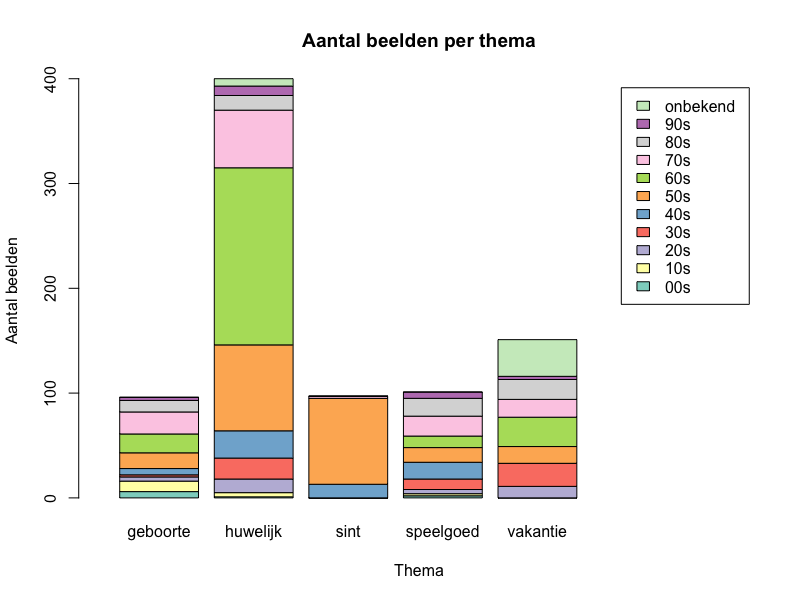
\includegraphics[width=\textwidth]{aantal_beelden_thema.png}\hfill
	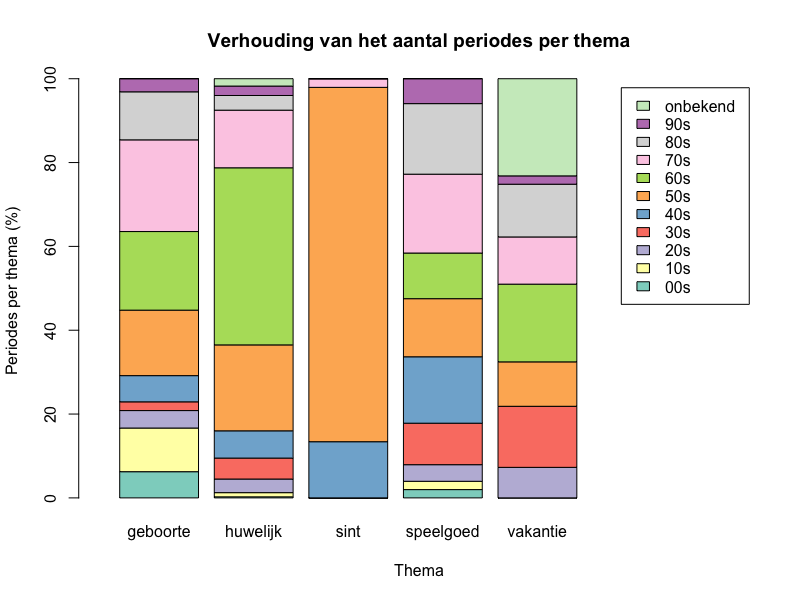
\includegraphics[width=\textwidth]{periode_per_thema.png}\hfill
	\caption[Staafdiagrammen met het aantal beelden per thema en de verhouding van het aantal periodes per thema]{\textbf{Boven:} Het aantal beelden per thema met opsplitsing van de beelden per periode (boven). Het aantal huwelijksfoto's springt er duidelijk uit. \textbf{Onder:} de verhouding van het aantal periodes per thema. Ook hier is het duidelijk dat dit ongelijk verdeeld is.}
	\label{fig:verhouding-beelden-thema}
\end{figure}

Het valt hierbij op dat de dataset ongelijk verdeeld is:
\begin{itemize}

	\item bijna de helft van de dataset bestaat uit huwelijksfoto’s. De andere thema’s zijn meer gelijk verdeeld met grofweg honderd foto’s per thema. 
	\item daarenboven concentreren de huwelijksfoto’s zich op drie periodes. Bijna 75\% van de foto’s zijn afkomstig uit de periode 50s, 60s en 70s. 
	\item de Sinterklaasfoto’s zijn afkomstig uit slechts drie periodes (40s, 50s en 70s) waarvan bijna 85\% uit één periode (50s).
	\item de ongelijke verdeling van de foto’s per thema heeft ook een gevolg op de foto’s per periode. Er zijn vooral foto’s afkomstig uit de periodes 50s, 60s en 70s. Voor 50s gaan bijna 80\% van de foto’s over huwelijk en Sinterklaas, voor de 60s bijna 75\% over huwelijk en voor de 70s zijn 50\% huwelijksfoto’s. Van de vroegste periodes (00s en 10s) zijn dan weer weinig foto’s (zie ook figuur \ref{fig:aantal-beelden-periode}).
	\item zowel Sinterklaas- als vakantiefoto’s komen niet in alle periodes voor.
\end{itemize}

Bij het interpreteren van de resultaten moet rekening gehouden worden met deze ongelijke verdeling.

\section{Keuze voor API}
\label{sec:keuze-voor-api}

Clarifai werd als API gekozen om de onderzoeksvraag te beantwoorden. 

Clarifai is opgericht in 2013 door Matthew Zeiler. Hij had in 2013 deelgenomen aan de ImageNet Challenge als doctoraatsstudent samen met zijn promotor Dr. Rob Fergus. Hun architectuur, ZFNet, waarop ook Clarifai gebouwd is, was de winnaar van de ImageNet Challenge~\autocite{Tsang2018}.

De keuze viel op deze API om een aantal redenen:
\begin{enumerate}
	\item De website bevat goede en duidelijke documentatie om met de API aan de slag te gaan. De uitleg wordt telkens voorzien van een voorbeeld in de ondersteunde programmeertalen.
	\item De API heeft clients in verschillende programmeertalen die het de ontwikkelaar mogelijk maken om de API te gebruiken in de programmeertaal naar keuze. JavaScript, Python, Java, C\# en PHP hebben officiële clients die door Clarifai ondersteund en ontwikkeld worden. De REST API kan ook rechtstreeks bevraagd worden zonder gebruikt van een API client~\autocite{ClarifaiAPI}.
	\item De Clarifai website beschikt over een grafische interface waarin gebruikers beelden kunnen opladen om ze te laten taggen door een van de ingebouwde modellen of een nieuw model kunnen trainen. Dit verhoogt het gebruiksgemak, wat, zoals besproken in~\ref{sec:probleemstelling}, een belangrijke factor was bij de keuze voor een API.
	\item Er zijn verschillende ingebouwde modellen die gebruikt kunnen worden om beelden te taggen, gaande van zeer algemene modellen (het general model) tot zeer specifieke modellen, zoals een model om modeconcepten te herkennen of een model om elementen met betrekking tot voeding en vaatwerk te detecteren.
\end{enumerate}

\section{Beelden beschikbaar maken via een publieke URL}
\label{sec:beelden-via-URL}

Het Huis van Alijn bracht ons de beelden aan op een harde schijf. De beelden waren immers nog niet online beschikbaar. Om op een geautomatiseerde manier de API van Clarifai te kunnen bevragen, moest een publieke URL voor de beelden voorzien worden. Het waren hoge resolutie beelden waarvan het merendeel in TIFF-formaat was en een kleiner deel in JPEG-formaat. De meeste beelden hadden daarom een bestandsgrootte (10 \'{a} 13 MB per beeld) die te groot is voor Clarifai. Clarifai wil immers beelden met een grootte van maximum 3,6 MB. 

De beelden werden daarom op een beeldenserver geplaatst waarmee met een URL het beeld opgevraagd kon worden in een kleinere bestandsgrootte in het JPEG-bestandsformaat. Clarifai kan immers niet omgaan met beelden groter dan 3,6 MB. Een andere optie was om de beelden te converteren naar JPEG, ze daarbij te verkleinen naar een breedte van 512 pixels en ze vervolgens op een webserver of FTP-server te plaatsen. Clarifai verkleint immers zelf alle beelden tot 512 pixels en hoe dichter je bij dat formaat komt, hoe sneller de API calls verlopen~\autocite{Clairbot2019}. Dit laatste ontdekten we echter pas nadat de test al uitgevoerd was. Het was namelijk niet opgenomen in de documentatie.

De beelden werden opgeladen in een Amazon AWS EC2 Ubuntu instance waarop de beeldenserver (Cantaloupe) ge\"{i}nstalleerd was. Op die manier kreeg ieder beeld een publieke URL die gebruikt kon worden bij het aanroepen van de Clarifai API.

\section{Beschikbare metadata verzamelen in een CSV}
\label{sec:metadata-verzamelen-csv}

De 845 beelden van Huis van Alijn waren voorzien van metadata die uit de bestandsnaam van de digitale bestanden gehaald konden worden. Er werd een CSV gecreëerd waarin alle beschikbare metadata per beeld verzameld werden:
\begin{itemize}
	\item bestandsnaam of ID van het beeld;
	\item de extensie of het oorspronkelijke bestandsformaat van het beeld: .tif of .jpg;
	\item type: foto, diapositief of onbekend;
	\item thema;
	\item periode (decennium)
\end{itemize}

Op de harde schijf waren de afbeeldingen verzameld in een mapje (directory) per thema. Informatie zoals extensie, type, thema en periode werden uit de bestandsnaam gehaald.

\begin{lstlisting}[language=json,caption=een fragment van de CSV. De bestandsnaam heeft de logica \textit{type-periode-nr} waaruit onder meer de periode gehaald kan worden.]
filename,extension,type,theme,period
DIA-80-00249,tif,diapositief,vakantie,80s
DIA-80-00358,tif,diapositief,huwelijk,80s
DIA-90-00009,tif,diapositief,vakantie,90s
FO-00-00015,tif,foto,geboorte,00s
FO-00-00034,tif,foto,huwelijk,00s
\end{lstlisting}

\section{Uitvoeren van workflows}
\label{sec:uitvoeren-workflows}

Er werden twee workflows een aantal keer doorlopen bij het uitvoeren van dit onderzoek:
\begin{itemize}
	\item een workflow om de beelden te laten taggen door Clarifai;
	\item een workflow om via training een custom model te cre\"{e}ren.
\end{itemize}

\subsection{Workflow 1: Een dataset laten taggen door Clarifai}
\label{subsec:workflow1}

\subsubsection{De Clarifai API aanroepen}
\label{(subsubsec:clarifai-aanroepen)}

Clarifai beschikt over API-clients in verschillende programmeertalen (Java, Python, Javascript, C\#, Objective-C en PHP), maar doordat we zelf het meeste voeling hebben met shell scripting, werd gekozen om de REST API te bevragen via cURL, een command-line programma voor het verkrijgen of verzenden van bestanden met behulp van  een URL.

Een API key is nodig om de API te bevragen. Daarom werd eerst een account bij Clarifai aangemaakt. Automatisch verkrijg je dan een gratis key. 

Het general model van Clarifai werd gebruikt om de volledige dataset van Huis van Alijn te taggen. Dit is namelijk het meest uitgebreide model met de meeste concepten. het bevat ongeveer 11.000 verschillende concepten waaronder objecten, thema's, emoties in verschillende talen. Daardoor kan het model gebruikt worden voor een reeks van zeer uiteenlopende beelden~\autocite{ClarifaiGeneral}.

Om via de Clarifai API tags te krijgen voor een beeldbestand, moet commando \ref{lst:script-clarifai-aanroepen} ingegeven worden in de command line. \$\{API\_key\} en \$\{url\_naar\_het\_beeld\} moeten vervangen worden door respectievelijk de API key en de URL van het beeld. In de URL moet je verwijzen naar de id van het model en de id van de versie van het model die je wenst te gebruiken.~\autocite{ClarifaiAPI}. Voor het general model is dit \texttt{aaa03c23b3724a16a56b629203edc62c} en \texttt{aa7f35c01e0642fda5cf400f543e7c40}.

\begin{lstlisting}[language=bash,caption={bash commando om een beeld door Clarifai te laten taggen.}, label=lst:script-clarifai-aanroepen]
#!/bin/bash
curl -X POST
    -H 'Authorization: Key "${API_key}"'
    -H 'Content-Type: application/json'
    -d '{
        "inputs": [{
            "data": {
                "image": { 
                    "url": "'"${url_naar_het_beeld}"'"
                    }
                }
            }
        ]
    }'
"https://api.clarifai.com/v2/models/${model_id}/versions/${version_id}/outputs"
\end{lstlisting}

Het bevragen van de API verliep vlot. Gemiddeld waren er per beeld twee à drie seconden nodig. Bij drie beelden mislukte het aanroepen omdat ze een te groot bestandsgrootte hadden. Deze beelden werden verkleind waarna de API opnieuw aangeroepen werd.

\subsubsection{Tags van API in een overzicht verzamelen}
\label{subsubsec:tags-verzamelen-overzicht}

Na het bevragen van de Clarifai API werd per beeld een API response in JSON ontvangen met daarin onder meer de tags die aan de beelden gegeven werden.

\begin{lstlisting}[language=json,caption=een ingekorte versie van een ontvangen API response met voorspellingen van Clarifai .]
{
  "status": {
    "code": 10000,
    "description": "Ok",
    "req_id": "7a70efb773234ba9a3eaf219328782b4"
  },
  "outputs": [{
    "id": "94b039d533454d53b01f2d3f825a097e",
    "status": {
      "code": 10000,
      "description": "Ok"
    },
    "created_at": "2019-04-01T16:14:28.886109228Z",
    "model": {
      "id": "aaa03c23b3724a16a56b629203edc62c",
      "name": "general",
      "created_at": "2016-03-09T17:11:39.608845Z",
      "app_id": "main",
      "output_info": {
        "message": "Show output_info with: GET /models/{model_id}/output_info",
        "type": "concept",
        "type_ext": "concept"
      },
      "model_version": {
        "id": "aa7f35c01e0642fda5cf400f543e7c40",
        "created_at": "2018-03-06T21:10:24.454834Z",
        "status": {
       	  "code": 21100,
          "description": "Model trained successfully"
        }
      },
      "display_name": "General"
   	},
    "input": {
      "id": "d74a5f9d8961406eb5a15e9172be9399",
      "data": {
        "image": {
          "url": "http://ec2-18-191-252-182.us-east-2.compute.amazonaws.com:8182/iiif/2/FO-30-00197/full/full/0/default.jpg"
        }
      }
    },
    "data": {
      "concepts": [{
        "id": "ai_l8TKp2h5",
        "name": "people",
        "value": 0.999308,
        "app_id": "main"
      },{
        "id": "ai_bmls4LpL",
        "name": "group",
        "value": 0.9847269,
        "app_id": "main"
      },{
        "id": "ai_sd6DKdXp",
        "name": "group together",
        "value": 0.9833066,
        "app_id": "main"
      },{
        "id": "ai_RQccV41p",
        "name": "woman",
        "value": 0.9795268,
        "app_id": "main"
      },{
        "id": "ai_VPmHr5bm",
        "name": "adult",
        "value": 0.97893196,
        "app_id": "main"
      }]
    }
  }]
}
\end{lstlisting}

De gegevens werden verzameld in een CSV-bestand die geïmporteerd werd in Google Sheets. Google Sheets heeft als voordeel dat resultaten eenvoudig gedeeld kunnen worden met de museummedewerkers en bezit bovendien over ingebouwde reken- en queryfuncties die het analyseren van de resultaten vereenvoudigen. Bovendien kan Google Sheets afbeeldingen in een cel tonen via de \texttt{IMAGE}-functie\footnote{Voor meer info over de IMAGE-functie in Google Sheets, zie: \url{https://support.google.com/docs/answer/3093333?hl=en}}. Dit maakt het veel eenvoudiger om de gegevens te valideren.


\subsubsection{Gegevens valideren}
\label{subsubsec:gegevens-valideren}

Om de kwaliteit van de tags te controleren, werd dezelfde methodologie gebruikt als in \textcite{Vanstappen2019}. Bij ieder tag werd een checkbox geplaatst die door de validator aangevinkt moest worden indien de tag correct was. Dit had als voordeel dat de validatie relatief snel kon gebeuren en dat ook het verwerken van de resultaten eenvoudig was. 

Tijdens het valideren bleek het aanvinken van correcte tags niet altijd eenvoudig te zijn. Sommige tags vereisten enige interpretatie die moeilijk is zonder de context van het beeld te kennen. Het gaat om tags zoals \textit{happy}, \textit{music} en \textit{love}. Daarvoor konden we ons baseren op de thema’s van de foto’s. We gingen ervan uit dat mensen op huwelijksfoto’s en geboortefoto’s vol liefde waren, en dat zij, net als mensen op vakantie, gelukkig zijn. 

Een andere moeilijkheid was het herkennen van het geslacht van jonge kinderen op (oudere) foto's, of weten wanneer de mensen op de foto beschouwd konden worden als bejaard. We zijn bij het corrigeren van deze tags niet te streng geweest. Bij twijfel, wanneer bijvoorbeeld zowel de tags \textit{boy} als \textit{girl} voorkwamen, hebben we steeds de term met de grootste waarschijnlijkheidsscore goedgekeurd.

Ten slotte waren er ook nog de tags \textit{group}, \textit{several} en \textit{many}. We beschouwden een groep als een groep als er drie of meer mensen op de foto stonden. De andere tags werden gevoelsmatig goed- of afgekeurd.

\begin{figure}
	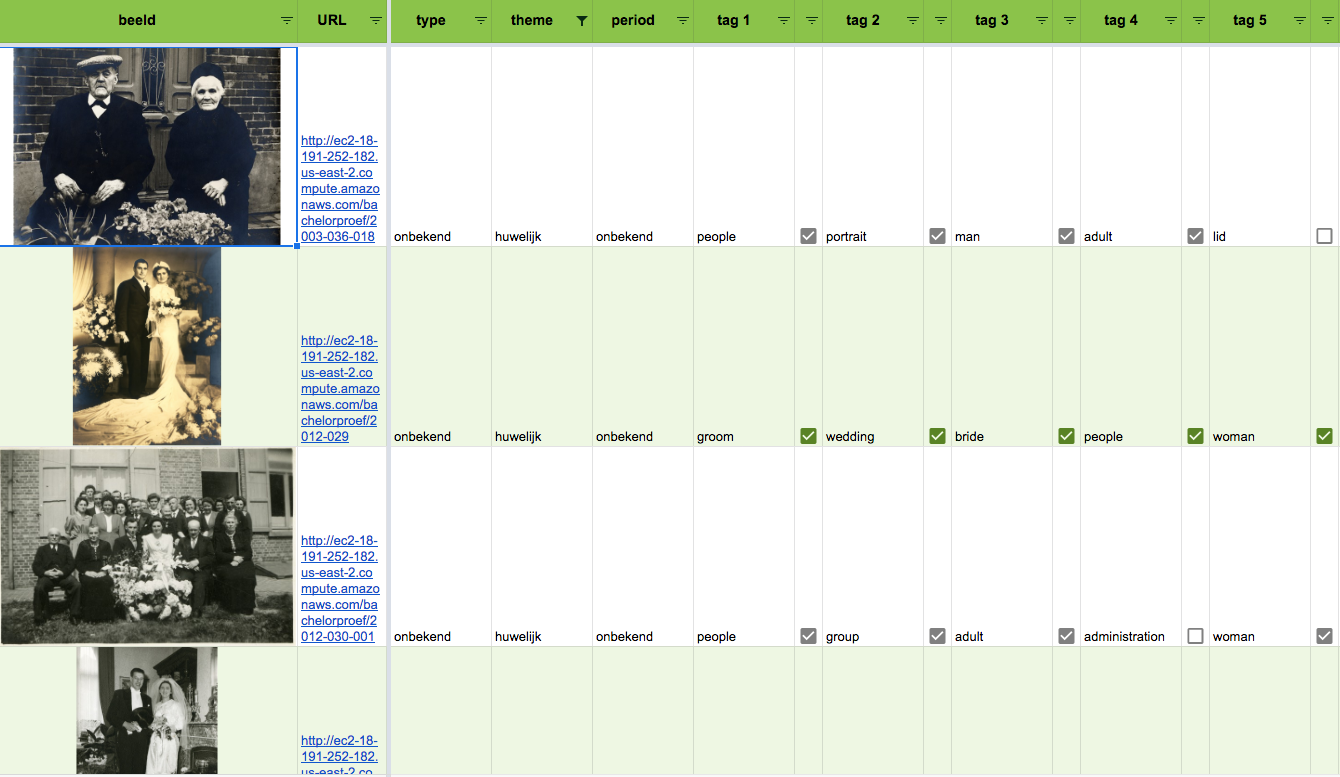
\includegraphics[width=\textwidth]
	{validatiescherm.png}
	\caption{Validatie van het ingebouwd model in Google Sheets.}
	\label{fig:validatiescherm}
\end{figure}

\subsection{Workflow 2: Een custom model trainen}
\label{subsec:workflow2}

Voor het trainen van de API door de creatie van een custom model werd de workflow gevolgd van \textcite{ClarifaiAPI}. Voor dit onderzoek werden twee custom models gemaakt:
\begin{itemize}
	\item een model die de beelden van Huis van Alijn kan classificeren volgens hun thema (geboorte, huwelijk, Sinterklaas, speeldgoed en vakantie), vanaf nu het themamodel;
	\item een model die de beelden van Huis van Alijn kan classificeren volgens het decennium waarin de foto getrokken was (1900s t.e.m. 1990s), vanaf nu het periodemodel.
\end{itemize}

Voor ieder model werden een aantal stappen doorlopen:
\begin{enumerate}
	\item het maken van een trainingsset en validatieset;
	\item het opladen van de trainingsbeelden naar Clarifai;
	\item het creëren van een custom model met de concepten uit de trainingsbeelden;
	\item het trainen van het model;
	\item het valideren van het model met de validatieset.
\end{enumerate}

De getrainde modellen werd vervolgens gebruikt om de hele dataset van Huis van Alijn te classificeren in respectievelijk thema en periode. 

Het is in Clarifai mogelijk om een custom model te maken via de API of via een webinterface. Voor dit onderzoek hebben we gebruik gemaakt van de API.

\subsubsection{Training- en validatieset maken}

Uit de dataset van Huis van Alijn werd een trainingset en een validatieset gemaakt. De trainingsbeelden dienden om het model te trainen; de validatiebeelden om de verschillende iteraties van het model te valideren en te beoordelen welke iteratie het meest performant is~\autocites{Lievens2017}{Brownlee2017}. Door de kleine dataset (845 beelden) wilden we slechts 50\% van de beelden gebruiken voor training; 20\% werd gebruikt als validatieset.

Trainingsbeelden en validatiebeelden werden willekeurig geselecteerd uit de dataset. \textcite{Gong2017} meldt dat het erg belangrijk is dat de trainingsbeelden overeenkomen met de beelden waarop het model toegepast zal worden. Er werd daarom gezorgd dat, in de mate van het mogelijke, in de beelden voor respectievelijk het themamodel en het periodemodel alle decennia en thema’s (gelijkmatig) aanwezig waren. Omdat een huwelijk in de jaren 1900 er nu eenmaal anders uitziet dan dat in de jaren 1950 of 1990 is het immers belangrijk dat het model zoveel mogelijk beelden te zien krijgt van hoe een huwelijk eruit kan zien doorheen alle periodes. Het periodemodel moet dan weer weten dat een foto uit een bepaald decennium kan bestaan uit zowel huwelijks-, geboorte-, Sinterklaas-, speelgoed- als vakantiefoto’s.

Voor het themamodel wilden we ieder thema evenwaardig trainen en dus evenveel trainingsbeelden per thema gebruiken. Doordat het aantal beelden per thema ongelijk verdeeld is (vierhonderd huwelijksfoto’s, $\pm$ honderd beelden voor de andere thema’s, zie tabel \ref{tab:analyse-dataset}), beslisten we om het aantal foto’s per thema te beperken tot honderd. Dit hield in dat voor ieder thema slechts vijftig foto’s gebruikt zouden worden als trainingsbeelden en dat de validatieset uit twintig foto’s per thema bestaat. 

Bij het periodemodel was het niet mogelijk om iedere periode evenwaardig te trainen. Het aantal beelden per decennium was hiervoor te ongelijk verdeeld (zie figuur \ref{fig:aantal-beelden-periode}). Er waren bijvoorbeeld minder dan dertig foto’s voor de jaren 00, 10 en 90, en meer dan tweehonderd foto’s voor de jaren 50 en 60. Beperken van het aantal foto’s per periode was daardoor onmogelijk. De trainingset zou dan  te marginaal zijn.

\begin{figure}
	\centering
	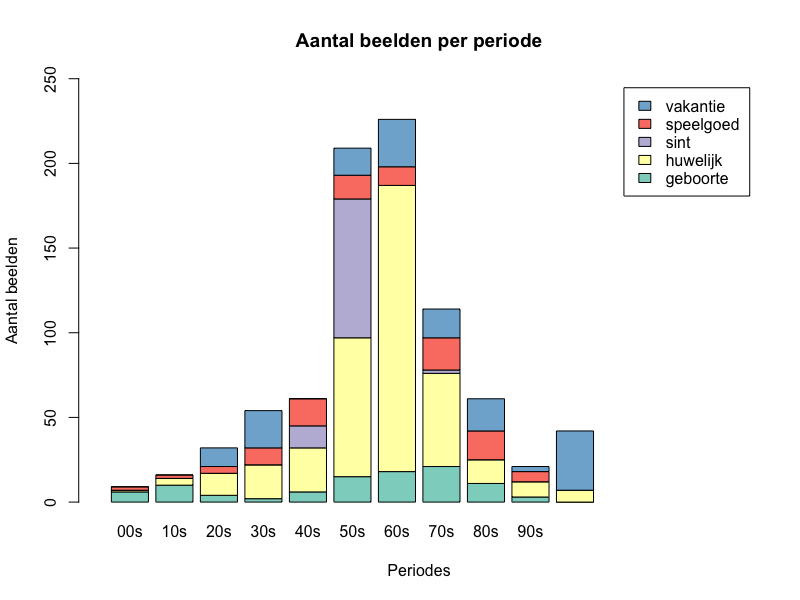
\includegraphics[width=\textwidth]{aantal_beelden_periode.png}\hfill
	\caption[Staafdiagram met het aantal beelden per periode]{Staafdiagram die het aantal beelden per periode weergeeft. De meest rechtse staaf toont het aantal beelden waarvan de periode niet gekend is.}
	\label{fig:aantal-beelden-periode}
\end{figure}


\subsubsection{Trainingsbeelden opladen naar de computer vision service}
\label{subsubsec:trainingsbeelden-opladen}

Om een model te maken, moeten eerst trainingsbeelden opgeladen worden die reeds het concept bevatten waarvan we willen dat het model het herkent~\autocite{ClarifaiAPI}. 

\begin{figure}[h]
	\centering
	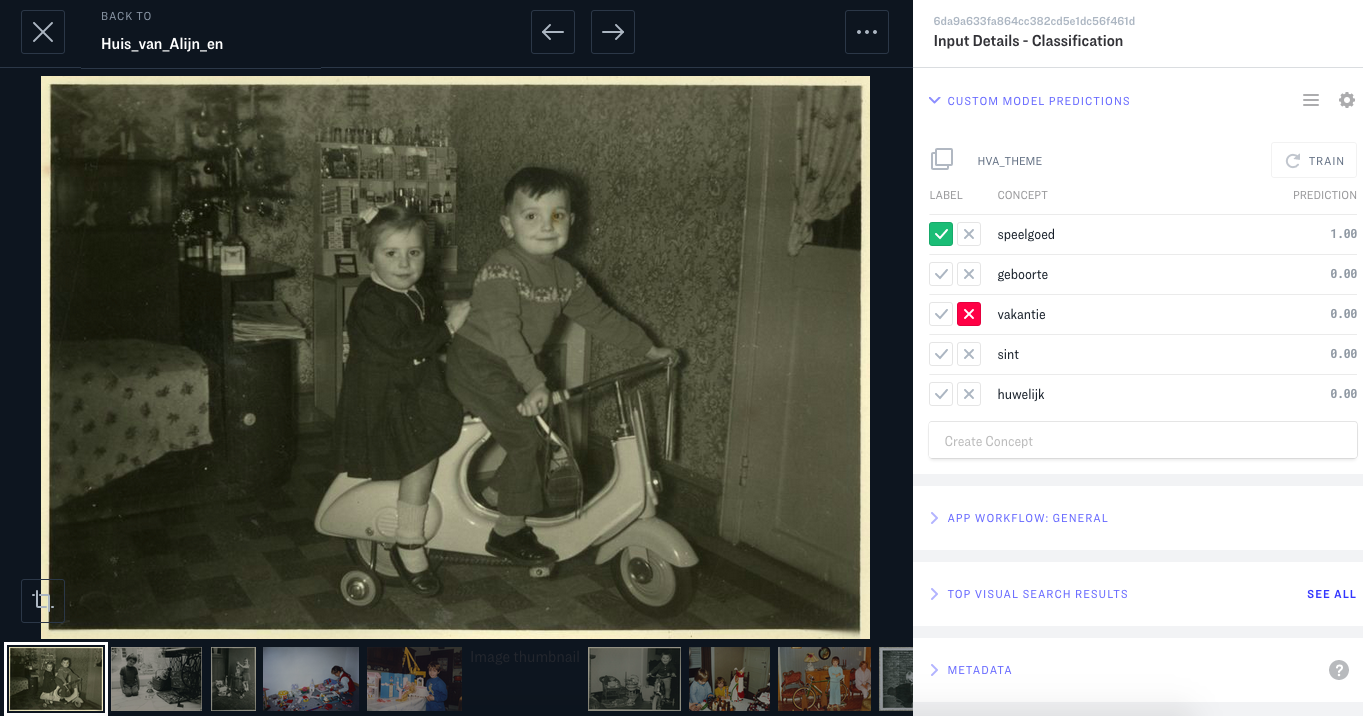
\includegraphics[width=\textwidth]{training_concept.png}\hfill
	\caption[Trainingsbeelden toevoegen via de webinterface]{Trainingsbeelden kunnen via de webinterface van Clarifai opgeladen en voorzien worden van een of meerdere concepten.}
	\label{fig:trainingsbeelden-toevoegen}
\end{figure}

We beslisten om het model in iteraties te trainen. \textcite{ClarifaiAPI} stelt immers voor om te starten met tien beelden per concept en vervolgens meer beelden per concept toe te voegen indien dit nodig blijkt. Na iedere iteratie werd het model gevalideerd. Voor het themamodel werd gewerkt met iteraties van tien trainingsfoto’s per thema. Voor het periodemodel werd dit opgetrokken tot iteraties van maximum dertig trainigsfoto’s per periode\footnote{Waar mogelijk, voor de decennia 00s, 10s, 20s, 30s en 90s waren geen dertig trainingsbeelden beschikbaar.}, omdat het periodemodel een grotere variëteit aan beelden moet herkennen.

\begin{lstlisting}[language=bash,caption={bash commando om een beeld met een concept naar Clarifai op te laden.}]
#!/bin/bash
curl -X POST \
  -H 'Authorization: Key "${API_key}"' \
  -H 'Content-Type: application/json' \
  -d '{
    "inputs": [{
      "data": {
        "image": {
          "url": "'"${url_naar_het_beeld}"'"
        },
        "concepts":[{
          "id": "'"${concept}"'",
          "value": true
        }]
      }
    }]
  }'\
https://api.clarifai.com/v2/inputs
\end{lstlisting}

\begin{lstlisting}[language=json,caption={Het antwoord van de Computer Vision API in JSON na het opladen van een beeld met een concept}]
{
  "status": {
    "code": 10000,
    "description": "Ok",
    "req_id": "f8db86f0ff564086a6611c7dd34e91e3"
  },
  "inputs": [{
    "id": "153005f7c8b04d949356dc36c1bbbee9",
    "data": {
      "image": {
        "url": "http://ec2-18-191-252-182.us-east-2.compute.amazonaws.com:8182/iiif/2/2003-036-018/full/922,/0/default.jpg"
      },
      "concepts": [{
        "id": "huwelijk",
        "name": "huwelijk",
        "value": 1,
        "app_id": "1b9b01460b944923a9eb1578668d4ea6"
      }]
    },
    "created_at": "2019-07-13T13:57:15.569447471Z",
    "modified_at": "2019-07-13T13:57:16.399324215Z",
    "status": {
      "code": 30000,
      "description": "Download complete"
    }
  }]
}
\end{lstlisting}

Het is in Clarifai ook mogelijk om negatieve concepten toe te voegen. Dit zijn concepten die niet op de foto te zien zijn. Op een huwelijksfoto kan bijvoorbeeld aangeduid worden dat dit geen speelgoed-, vakantie-, geboorte- en Sinterklaasfoto is. Om te testen of negatieve concepten een invloed hebben op de resultaten van de validatieset, werd na de eerste iteratie voor alle trainingsbeelden alle negatieve concepten toegevoegd.

\begin{figure}[h]
	\centering
	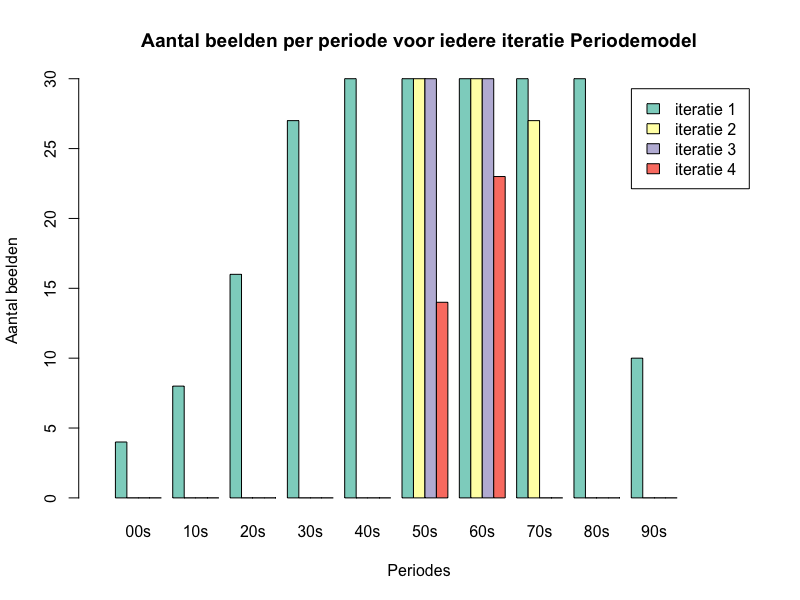
\includegraphics[width=\textwidth]{periodemodel_beelden_totaal.png}\hfill
	\caption[Het aantal beelden per periode voor iedere iteratie bij het trainen van het Periodemodel.]{Het aantal beelden per periode voor iedere iteratie bij het trainen van het Periodemodel.}
	\label{fig:periodemodel-iteraties}
\end{figure}


\subsubsection{Het model maken}
\label{subsubsec:model-maken}


Nadat de beelden van de eerste iteratie opgeladen werden naar Clarifai, kan het  het model aangemaakt worden. Aan het model moet een naam worden gegeven en de concepten toegevoegd die op de trainingsbeelden te zien zijn. 

Daarnaast kan het model nog geconfigureerd worden. In onze modellen werd ingesteld dat een beeld slechts één concept bevat\footnote{Een huwelijksfoto kan bijvoorbeeld nooit een vakantiefoto zijn.} (parameter \texttt{concepts\_mutually\_exclusive}) en dat er enkel trainingsbeelden gebruikt worden waarop een concept te zien is (parameter \texttt{closed\_environment})

\begin{lstlisting}[language=bash,caption=bash commando om een custom model met vijf concepten te creëren]
#!/bin/bash
curl -X POST \
  -H 'Authorization: Key "${API_key}"' \
  -H 'Content-Type: application/json' \
  -d '{
    "model": {
      "id": "HvA_theme",
      "output_info": {
        "data": {
          "concepts": [{
            "id": "'"${concept1}"'"
          },{
            "id": "'"${concept2}"'"
          },{
            "id": "'"${concept3}"'"
          },{
            "id": "'"${concept4}"'"
          },{
            "id": "'"${concept5}"'"
          }]
        },
        "output_config": {
          "concepts_mutually_exclusive": true,
          "closed_environment": true
        }
      }
    }
  }'\
  https://api.clarifai.com/v2/models
\end{lstlisting}

\begin{lstlisting}[language=json,caption=antwoord van de API na het creëren van het model]
{
  "status": {
    "code": 10000,
    "description": "Ok",
    "req_id": "66be8c1a7bbc4cca9398d02c7c15a097"
  },
  "model": {
    "id": "HvA_theme",
    "name": "HvA_theme",
    "created_at": "2019-07-13T14:15:49.966900528Z",
    "app_id": "1b9b01460b944923a9eb1578668d4ea6",
    "output_info": {
      "output_config": {
        "concepts_mutually_exclusive": true,
        "closed_environment": true,
        "max_concepts": 0,
        "min_value": 0,
        "test_split_percent": 10
      },
      "message": "Show output_info with: GET /models/{model_id}/output_info",
      "type": "concept",
      "type_ext": "concept"
    },
    "model_version": {
      "id": "68b9e3c20ae04abbbdc2e3fb974b9a0f",
      "created_at": "2019-07-13T14:15:49.994520471Z",
      "status": {
        "code": 21102,
        "description": "Model not yet trained"
      },
      "active_concept_count": 5
    }
  }
}
\end{lstlisting}

\begin{figure}[h]
	\centering
	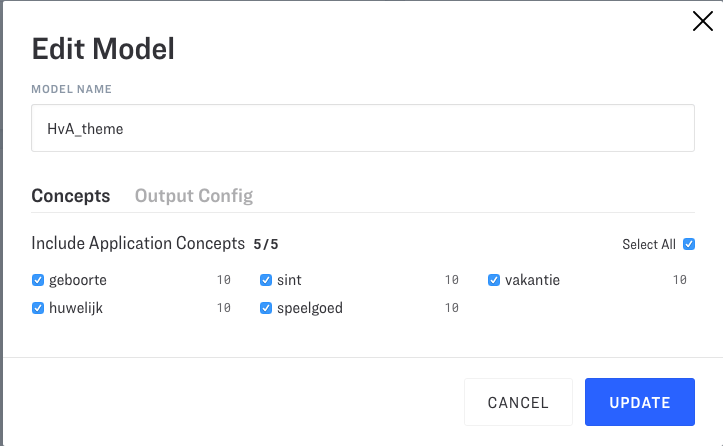
\includegraphics[width=\textwidth]{train_create_model.png}\hfill
	\caption[Een model maken via de webinterface]{Een custom model kan via de webinterface van Clarifai gecreëerd en aangepast worden.}
	\label{fig:model-maken}
\end{figure}


\subsubsection{Het model trainen}
\label{subsubsec:model-trainen}

Telkens er nieuwe trainingsbeelden toegevoegd zijn, moet het model getraind worden. Door het trainen van het model gaat het systeem naar alle beelden met de concepten kijken en daarvan leren~\autocite{ClarifaiAPI}. 


\begin{lstlisting}[language=bash,caption=bash commando om het model te trainen]
#!/bin/bash
curl -X POST \
  -H 'Authorization: Key "${API_key}"' \
  -H 'Content-Type: application/json' \
  "https://api.clarifai.com/v2/models/${model_id}/versions" 
\end{lstlisting}

\begin{lstlisting}[language=json,caption=antwoord van de API nadat het model getraind werd]
{
  "status": {
    "code": 10000,
    "description": "Ok",
    "req_id": "2f513295f4074ec39115e3e5e500d652"
  },
  "model": {
    "id": "HvA_theme",
    "name": "HvA_theme",
    "created_at": "2019-07-13T14:15:49.966900Z",
    "app_id": "1b9b01460b944923a9eb1578668d4ea6",
    "output_info": {
      "output_config": {
        "concepts_mutually_exclusive": true,
        "closed_environment": true,
        "max_concepts": 0,
        "min_value": 0,
        "test_split_percent": 10
      },
      "message": "Show output_info with: GET /models/{model_id}/output_info",
      "type": "concept",
      "type_ext": "concept"
    },
    "model_version": {
      "id": "b6fd2a1befd947bdb200b5e635721657",
      "created_at": "2019-07-13T14:28:25.060240688Z",
      "status": {
        "code": 21103,
         "description": "Custom model is currently in queue for training, waiting on inputs to process."
      },
      "active_concept_count": 5
    }
  }
}
\end{lstlisting}

\begin{figure}[h]
	\centering
	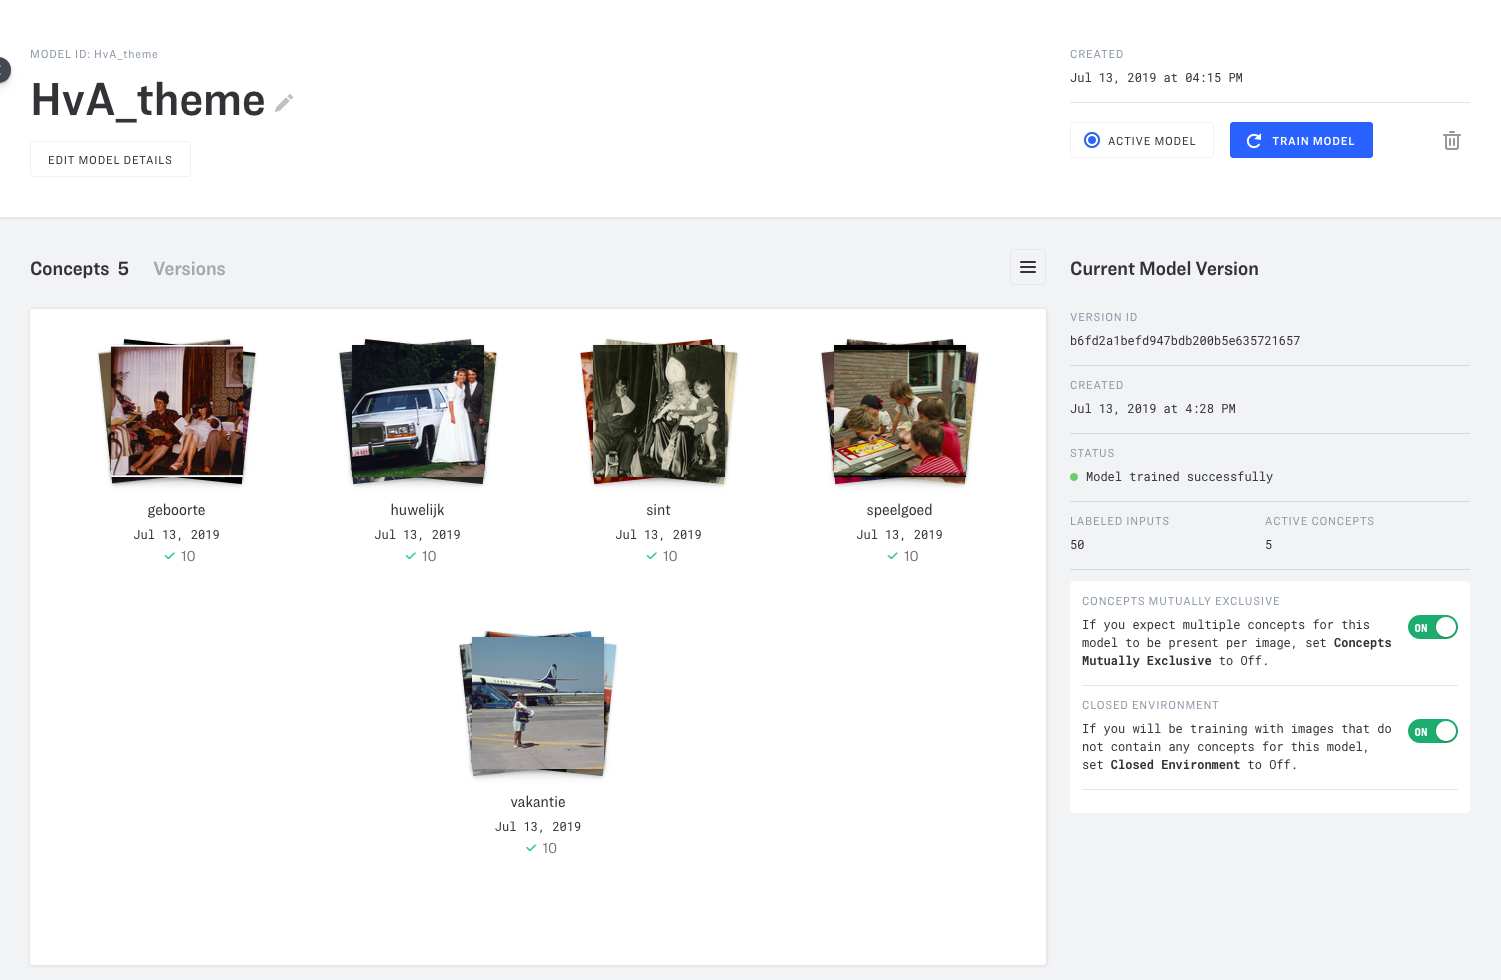
\includegraphics[width=\textwidth]{train_model.png}\hfill
	\caption[Het model trainen via de webinterface]{Het model kan via de webinterface van Clarifai getraind worden.}
	\label{fig:model-trainen}
\end{figure}

Na het trainen krijgt het model een versiecode. Met deze code is het mogelijk om bij het voorspellen een bepaalde versie van het model te gebruiken. Als blijkt dat het model na iteratie 3 beter is dan dat van iteratie 4, dan kan je met de versiecode het model van iteratie 3 gebruiken.

\subsubsection{Het model valideren}
\label{subsubsec:model-valideren}

Nadat het model getraind was, werd het uitgetest op de validatieset. Hiervoor werd workflow 1 uit \ref{subsec:workflow1} doorlopen met de validatiesets voor de twee modellen.

\begin{figure}
	\centering
	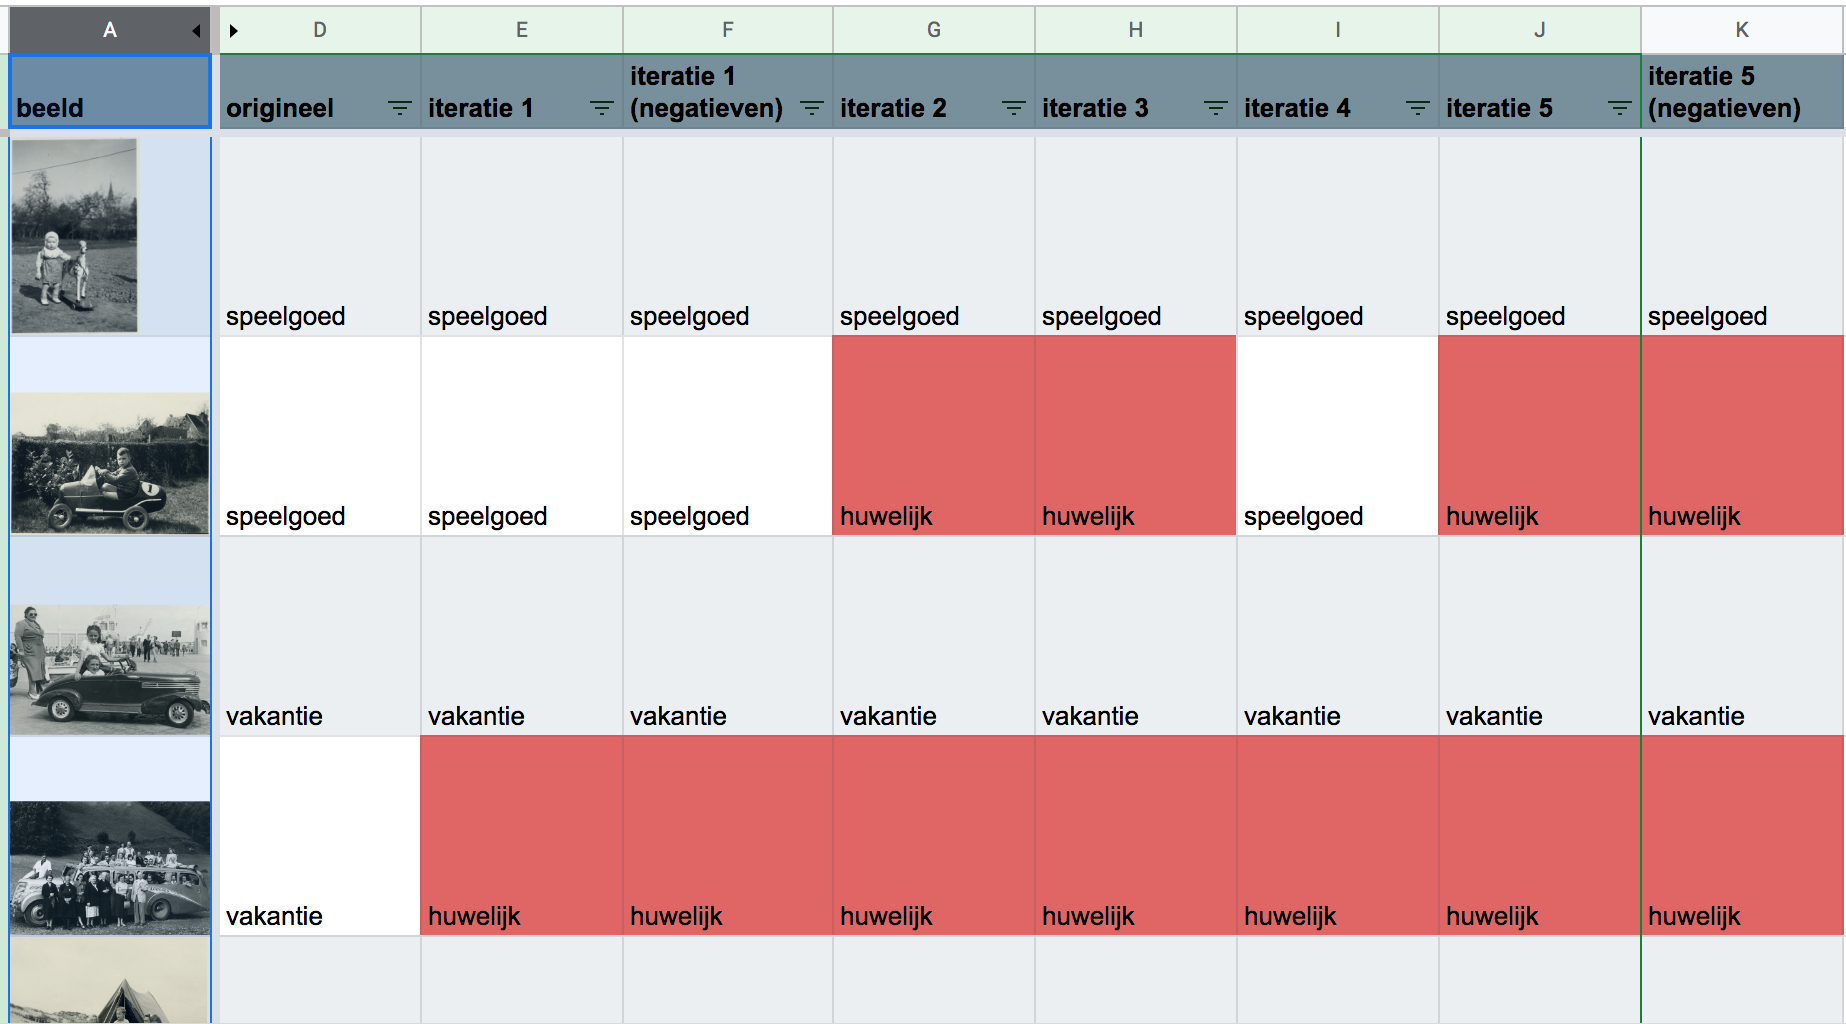
\includegraphics[width=\textwidth]{validatie_model.png}\hfill
	\caption{Validatie van het custom model in Google Sheets.}
	\label{fig:validatie-model}
\end{figure}

Om het model te beoordelen werd gebruik gemaakt van de gemiddelde rappel, precisie en \textit{F$_{1}$}-score~\autocites{Lievens2017}{Koehrsen2018}:
\begin{itemize}
    \item De rappel is het percentage van de positieve trainingsbeelden die ook effectief als positief werd gelabeld door het model (verhouding tussen het aantal true positives en het totaal aantal positieve voorbeelden van het concept);
    \item De precisie is het percentage van de beelden die als een bepaald concept herkend werken daadwerkelijk dat concept bevatten (verhouding tussen het aantal true positives en het totaal aantal herkende beelden voor dat concept);
    \item De precisie en de rappel kunnen gecombineerd worden in één enkele score, de $F_1$-score. Dit is het harmonisch gemiddelde van beide cijfers. Om een grote $F_1$-score te behalen moeten bijgevolg zowel de precisie als de rappel het goed doen.\footnote{~Formule voor het verkrijgen van de $F_1$-score: $F_1 = 2 \cdot \frac{\mathrm{precisie} \cdot \mathrm{rappel}}{\mathrm{precisie} + \mathrm{rappel}}$}
\end{itemize}

Hoe groter deze scores, hoe performanter het model. Clarifai geeft meerdere concepten aan een model. Er werd enkel rekening gehouden met het concept dat de hoogste waarschijnlijkheidsscore gekregen heeft. Hierbij werd geen drempelwaarde ingesteld. Dit betekent dat als aan een beeld een correct concept toegekend werd met een waarschijnlijkheid van 10\%, dat deze ook als een true positive bestempeld werd. 

De hoogste $F_1$-score voor het Themamodel werd behaald in de vierde iteratie met een score van 92\% (tabel \ref{tab:validatie-themamodel}). In de vijfde iteratie daalt de score licht tot 91\%. Na de eerste iteratie (tien trainingsbeelden voor ieder thema) werd er al een $F_1$-score van 78\% behaald. Het toevoegen van veertig negatieve voorbeelden na de eerste iteratie zorgde voor een lichte stijging tot 80\%. Als de vierde iteratie van naderbij bekeken wordt (tabel \ref{tab:validatie-iteratie4-themamodel}), dan valt het op dat het model erg goed is in het classificeren van de Sinterklaasfoto’s (score van 100\%). Het minst scoorde op de speelgoed- en geboortefoto’s met een $F_1$-score van respectievelijk 84\% en 85\%. Bij de speelgoedfoto’s werd een lagere rappel behaald (80\%), maar was de precisie hoger (89\%). 

\begin{table}
    \centering
    \renewcommand\arraystretch{1.2}
    \begin{tabular}{l|cc|c}
        \toprule
        & aantal positieven  &  aantal negatieven & $F_1$-score (\%)\\
        \midrule
        iteratie 1/A & 10 & 0 & 78 \\
        iteratie 1/B & 10 & 40 & 80 \\
        iteratie 2 & 20 & 40 & 86 \\
        iteratie 3 & 30 & 40 & 88 \\
        iteratie 4 & 40 & 40 & 92 \\
        iteratie 5 & 50 & 40 & 91 \\
        \bottomrule
    \end{tabular}
    \caption[De $F_1$-scores voor de verschillende iteraties van het Themamodel.]{De $F_1$-scores voor de verschillende iteraties van het Themamodel met vermelding van het aantal postieve en negatieve voorbeelden per thema na iedere iteratie.}
    \label{tab:validatie-themamodel}
\end{table}


\begin{table}
    \centering
    \renewcommand\arraystretch{1.2}
    \begin{tabular}{l|ccc|rrr}
        \toprule
        & true positives  & false negatives & false positives & rappel & precisie & $F_1$-score \\
        \midrule
        geboorte & 17 & 3 & 3 & 85\% & 85\% & 85\% \\
        huwelijk & 20 & 0 & 2 & 100\% & 91\% & 95\% \\
        Sint & 20 & 0 & 0 & 100\% & 100\% & 100\% \\
        speelgoed & 16 & 4 & 2 & 80\% & 89\% & 84\% \\
        vakantie & 19 & 1 & 1 & 95\% & 95\% & 95\% \\
        \midrule
        gemiddelde & 18,4 & 1,6 & 1,6 & 92\% & 92\% & 92\% \\
        \bottomrule
    \end{tabular}
    \caption{De resultaten (rappel, precisie en $F_1$-score) van de vierde iteratie bij het trainen van het Themamodel.}
    \label{tab:validatie-iteratie4-themamodel}
\end{table}

Bij het Periodemodel, met de onevenwichtige en beperkte trainingset, werd op de validatieset slechtst een maximale $F_1$-score van 48\% behaald na iteratie 2. Het valt op dat vanaf iteratie 3 de score weer daalt. Een mogelijke verklaring is dat het aantal trainingsbeelden per periode te verschillend is. De rappel en de precisie stijgen voor een beperkt aantal periodes, maar dalen voor alle andere periodes. Het toevoegen van negatieve voorbeelden na iteratie 1 brengt geen verandering in de rappel, precisie en $F_1$-score. Iteratie 1 en iteratie 1 met negatieven hebben beiden een F-score van 40\%. Iteratie 2 behaalde de grootste rappel voor beelden uit de jaren 40 (67\%) en de grootste precisie op beelden uit de jaren 10 (100\%). De grootste globale score werd behaald op beelden uit de jaren 80 met een F-score van 58\%. Het model scoorde het slechtst op foto’s uit het eerste decennium de jaren 1900 en de jaren 90, met een $F_1$-score van respectievelijk 0\% en 29\%. Dit zijn periodes met weinig trainingsbeelden (resectievelijk vier en tien). Het is opmerkelijk dat het model bij foto's van de jaren 10 toch een $F_1$-score van 50\% behaalt, terwijl deze periode ook maar acht trainingsbeelden heeft.

\begin{table}
	\centering
	\renewcommand\arraystretch{1.2}
	\begin{tabular}{l|cc|c}
		\toprule
		& aantal positieven  &  aantal negatieven &  $F_1$-score (\%)\\
		\midrule
		iteratie 1/A & 21,5 & 0 & 40 \\
		iteratie 1/B & 21,5 & 193,5 & 40 \\
		iteratie 2 & 30,2 & 193,5 & 48 \\
		iteratie 3 & 36,2 & 193,5 & 47 \\
		iteratie 4 & 39,9 & 193,5 & 44 \\
		\bottomrule
	\end{tabular}
	\caption[De $F_1$-scores voor de verschillende iteraties van het Periodemodel.]{De $F_1$-scores voor de verschillende iteraties van het Periodemodel met vermelding van het gemiddeld aantal positieve en negatieve voorbeelden per thema na iedere iteratie. Zie figuur \ref{fig:periodemodel-iteraties} om een beeld te hebben van de volledige spreiding van de trainingset}
	\label{tab:validatie-periodemodel}
\end{table}

\begin{table}
	\centering
	\renewcommand\arraystretch{1.2}
	\begin{tabular}{l|ccc|rrr}
		\toprule
		& true positives  & false negatives & false positives & rappel & precisie & $F_1$-score \\ 
		\midrule
		00s & 0 & 2 & 0 & 0\% & 0\% & 0\% \\ 
		10s & 1 & 2 & 0 &  33\% & 100\% & 50\% \\ 
		20s & 4 & 3 & 5 & 57\% & 44\% & 50\% \\ 
		30s & 5 & 5 & 12 & 50\% & 29\% & 37\% \\ 
		40s & 8 & 4 & 13  & 67\% & 38\% & 49\% \\ 
		50s & 15 & 23 & 15  & 39\% & 50\% & 44\% \\ 
		60s & 13 & 21 & 13  & 48\% & 59\% & 53\% \\ 
		70s & 12 & 9 & 12  & 55\% & 48\% & 51\% \\ 
		80s & 5 & 5 & 5  & 58\% & 58\% & 58\% \\ 
		90s & 2 & 3 & 2  & 25\% & 33\% & 29\% \\ 
		\midrule
		gemiddelde & 7,1 & 7,7 & 7,7  & 43\% & 46\% & 42\% \\ 
		\bottomrule
	\end{tabular} 
	\caption{De resultaten (rappel, precisie en $F_1$-score) van de tweede iteratie bij het trainen van het Periodemodel.}
	\label{tab:validatie-iteratie2-periodemodel}
\end{table}

Wat doet de scores dalen na een hogere iteratie? Bij het Periodemodel vermoedden we dat dit komt door het onevenwicht in het aantal trainingsbeelden tussen de verschillende periodes, maar voor het Themamodel is dit moeilijker te bepalen omdat de thema’s even goed getraind zijn. Misschien komt het door een licht onevenwicht in het aantal periodes in de trainingsbeelden van het themamodel? Bij iteratie 4 liggen de aantallen iets dichter op mekaar (met een uitschieter voor de jaren 50), terwijl in iteratie 5 de uitschieter van de jaren 50 nog groter geworden is. Ook bij het periodemodel zien we de verhouding tussen het aantal thema’s in de foto’s groter worden na iteratie 2. Dit moet verder onderzocht worden met grotere datasets om hier conclusies uit te trekken. Een andere mogelijkheid is dat we op de grenzen van de CV API gestoten zijn.


% Voeg hier je eigen hoofdstukken toe die de ``corpus'' van je bachelorproef
% vormen. De structuur en titels hangen af van je eigen onderzoek. Je kan bv.
% elke fase in je onderzoek in een apart hoofdstuk bespreken.

\chapter{Resultaten met het ingebouwd model}
\label{ch:resultaten-ingebouwd-model}

De 845 beelden van Huis van Alijn werden getagged door het general model van Clarifai. Aan iedere foto werden twintig tags gegeven. De waarschijnlijkheidsscore van de tags bevond zich tussen 100\% en 65\% en had een gemiddelde van 93\%. 

De verkregen tags zijn op te delen in een aantal categorieën en gaan over verschillende aspecten van het beeld:
\begin{itemize}
	\item entiteiten die op de beelden te zien zijn, waaronder \textit{volwassene}, \textit{speelgoed}, \textit{bloem}, \textit{kameel}, \textit{jurk}, \textit{meubels} en \textit{strand};
	\item activiteiten die uitgevoerd worden op de beelden, zoals \textit{dansen}, \textit{zitten}, \textit{rusten}, \textit{shoppen} en \textit{reizen};
	\item emoties of gevoelens die te zien zijn op het beeld of die opgeroepen worden door het beeld, denk aan \textit{plezier}, \textit{liefde}, \textit{genot}, \textit{avontuur}, \textit{affectie}, \textit{sexy} en \textit{mooi};
	\item maar ook contextuele concepten, zoals \textit{vriendschap}, \textit{familie}, \textit{toerisme}, \textit{vrije tijd} en \textit{het samen zijn};
	\item en hoeveelheden: \textit{één}, \textit{twee}, \textit{drie}, \textit{vier}, \textit{veel}, \textit{enkele}. Dit waren vaak weinigzeggende termen die opvallend vaak fout waren. Het was ook niet altijd duidelijk waar die hoeveelheden op sloegen. Veel mensen? Veel bloemen?
	\item tot slot kregen we ook informatie over de foto zelf: \textit{portret}, \textit{kleur}, \textit{zwart-wit}, \textit{sepia}, \textit{monochroom}...
\end{itemize}

Tijdens de validatie werd vastgesteld dat Clarifai veel algemene termen geeft, zoals \textit{mensen}, \textit{volwassene}, \textit{kind}, \textit{groep} en \textit{veel}, maar soms waren we ook verwonderd over de relevantie van de tags. Enkele van die relevante tags zijn: \textit{schildersezel}, \textit{roos}, \textit{uitstapje}, \textit{airbus}, \textit{souvenir}, \textit{bazaar}, \textit{grasland}, \textit{broche} en \textit{bruidsmeisje}. 

Na validatie bleken 11.517 van de 16.900 tags correct te zijn (68,15\%). Dit resulteerde in 371 unieke termen die de foto’s beschreven. Bij 21 foto’s waren alle twintig tags correct. 97 beelden (11,5\%) hadden minder dan tien correcte tags, waarvan de slechts scorende een foto is van het thema speelgoed. Deze foto had slechts zes juiste tags. Gemiddeld hadden de foto’s 13,6 correcte tags.

\begin{figure}
	\centering
	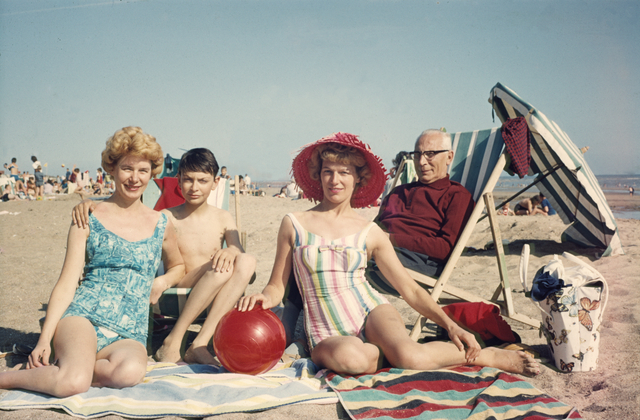
\includegraphics[width=0.495\textwidth]{DIA-0078-0352.jpg}\hfill
	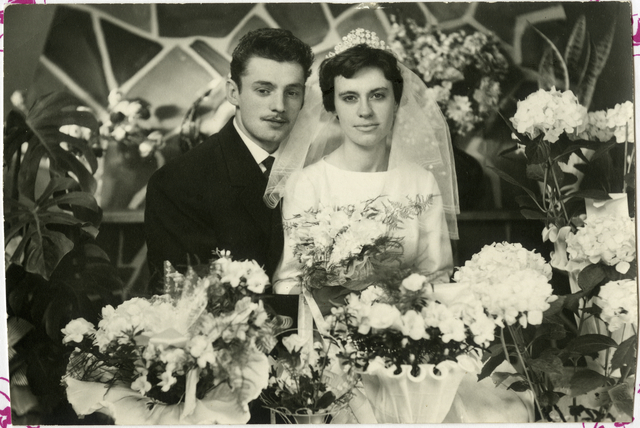
\includegraphics[width=0.495\textwidth]{FO-50-01658.jpg}\hfill
	\\[\smallskipamount]
	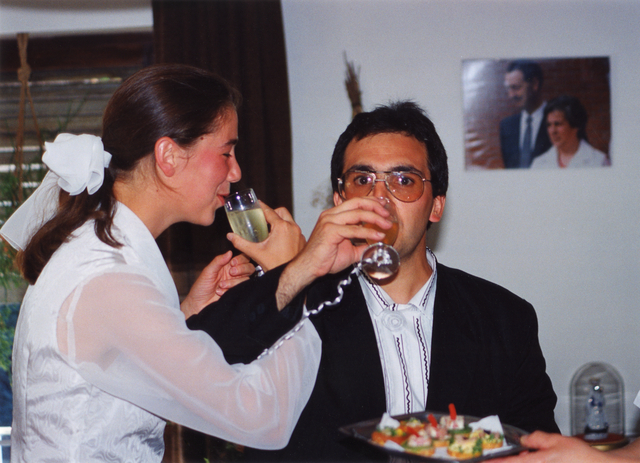
\includegraphics[width=0.57\textwidth]{FO-90-00157.jpg}\hfill
	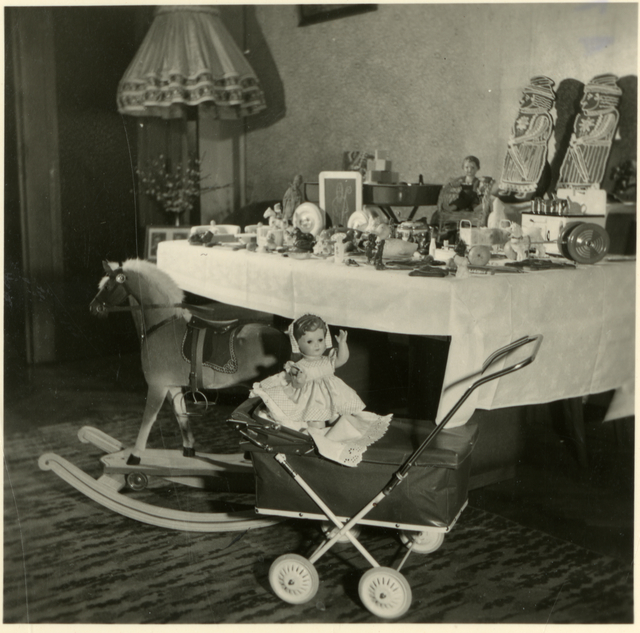
\includegraphics[width=0.42\textwidth]{FO-50-02073.jpg}\hfill
	\caption[Enkele voorbeelden van foto's die goed of slecht getagged werden door het ingbouwde Clarifai-model]{Drie foto’s uit de fotocollectie van Huis van Alijn waarvan alle tags correct waren en de foto waar het minst aantal tags correct waren (rechtsonder).}
\end{figure}

Vooraf hadden we verwacht dat het model niet goed zou scoren op de Sinterklaasfoto’s. Sinterklaas is immers een ritueel dat enkel voorkomt in de lage landen en enkele vroegere koloniën van Nederland. De kans lijkt dus klein dat het model de concepten van Sinterklaas kent. Omdat modellen voornamelijk getraind worden met hedendaagse foto’s, vreesden we ook dat de resultaten met de oudere foto’s minder goed zouden zijn.

%TODO referenties naar tabellen
Na validatie bleek het vermoeden rond de Sinterklaasfoto’s correct te zijn (zie tabel \ref{tab:analyse-resultaten-thema}). Het valt meteen op dat dit thema het laagste gemiddelde en het hoogst aantal foto’s met minder dan tien correcte tags heeft. Aan de beelden van dit thema werden tevens het minst aantal unieke termen gegeven. Het model blijkt ook minder goed op het speelgoedthema te scoren. De resultaten voor de huwelijksfoto’s zijn dan weer erg goed. Het gemiddelde voor dit thema is ongeveer 1,5 punten beter dan het gemiddelde van alle beelden.

%TODO captions van de foto' checken
	
\begin{table}
	\begin{tabular}{p{3cm}|ccccc}
	 	\toprule
		 & $\bar{x}$ (/20) & $\max$ & $\min$ & $\sharp$ unieke termen & $\sharp$ < 10 \\ 
		\midrule
		Geboorte & 13,69 & 20 & 7 & 112 & 7 \\ 
		Huwelijk & 15,16 & 20 & 8 & 158 & 7 \\ 
		Sint & 10,03 & 15 & 7 & 51 & 48 \\ 
		Speelgoed & 11,28 & 17 & 6 & 126 & 23 \\ 
		Vakantie & 13,42 & 20 & 9 & 212 & 12 \\ 
		Alle foto's & 13,63 & 20 & 6 & 371 & 97 \\ 
	\bottomrule
	\end{tabular} 
	\caption[een overzicht van de resultaten per thema na gebruikt van het ingebouwde model van Clarifai]{een overzicht van het gemiddelde ($\bar{x}$), maximale en minimale aantal juiste tags van de twintig tags van Clarifai voor de foto’s per thema, het aantal unieke termen dat gegeven werd aan ieder thema en het aantal foto’s waarvan minder dan tien tags correct waren. }
	\label{tab:analyse-resultaten-thema}
\end{table}

Wat betreft de periodes is het moeilijker om conclusies te trekken. Uit tabel \ref{tab:analyse-resultaten-periode} kan afgeleid worden dat de recentere foto’s (1960-1999) beter scoren en dat de oudste foto’s het slechtst scoren. Niettemin moet hier nuance van gemaakt worden. Er zijn immers slechts negen beelden uit de jaren 1900. Bovendien bestaan foto’s uit de jaren 50 - en in mindere mate uit de jaren 40 - voor een groot deel uit foto’s over Sinterklaas, wat hun slechtere score kan verklaren. Foto’s uit de jaren 60 scoren opmerkelijk goed, maar dit valt dan weer te verklaren door de grote aanwezigheid van huwelijksfoto’s in die periode (meer dan 75\%).\footnote{zie \ref{sec:analyseren-van-de-dataset}}

\begin{table}
	\begin{tabular}{p{3cm}|cccc}
		\toprule
		& $\bar{x}$ (/20) & $\max$ & $\min$ &  $\sharp$ < 10 \\ 
		\midrule
		00s & 11,44 & 14 & 9 & 1 \\ 
		10s & 12,69 & 16 & 8 &  2 \\ 
		20s & 12,91 & 19 & 9 & 3 \\ 
		30s & 13,26 & 20 & 9  & 3 \\ 
		40s & 12,16 & 20 & 7  & 19 \\ 
		50s & 12,33 & 20 & 6  & 48 \\ 
		60s & 15,01 & 20 & 7  & 7 \\ 
		70s & 14,56 & 20 & 7  & 4 \\ 
		80s & 14,26 & 20 & 7  & 3 \\ 
		90s & 14,48 & 20 & 9  & 1 \\ 
		Onbekend & 12,76 & 20 & 9  & 6 \\ 
		Alle foto's & 13,63 & 20 & 6  & 97 \\ 
		\bottomrule
	\end{tabular} 
	\caption[een overzicht van de resultaten per periode na gebruikt van het ingebouwde model van Clarifai]{een overzicht van het gemiddelde ($\bar{x}$), maximale ($\max$) en minimale ($\min$) aantal juiste tags van de twintig tags van Clarifai voor de foto’s per periode en het aantal foto’s waarvan minder dan tien tags correct waren. }
	\label{tab:analyse-resultaten-periode}
\end{table}

\section{Gedetailleerde resultaten per thema}
\label{sec:gedetailleerde-resultaten-per-thema}

In dit deel wordt dieper ingegaan op de resultaten per thema. Voor ieder thema wordt de top 30 van meest voorkomende termen, het maximale, minimale en gemiddeld aantal correcte tags, het aantal beelden met minder dan tien juiste tags en het aantal unieke termen toegelicht. 

\subsection{Geboorte}

In totaal waren er 96 beelden voor dit thema. De API scoorde goed op deze foto’s, in lijn met het totale gemiddelde. Er werden 112 unieke termen gebruikt om de beelden te beschrijven. Gemiddeld waren 13,7 tags correct. Het maximale aantal correcte tags was twintig, het minste zeven. Slechts zeven beelden hadden minder dan tien correcte tags (7,2\%).
\begin{table}
	\centering
	\begin{tabular}{*{3}{l}}
		\toprule
		mensen (93) & zoon (48) & gezichtsexpressie (22) \\
		volwassene (83) & 	groep (35) & meisje (19) \\
		kind (82) & twee (32) & affectie (17) \\
		vrouw (76) & sepia (29) & drie (16) \\
		portret (75) & binnenshuis (27) & verschillende (15) \\
		familie (65) & 	kamer (27) & broer of zus (13) \\
		kledij (62) & 	meubels (25) & bed (10) \\
		nageslacht (51) & liefde (25) & jongen (8) \\
		man (49) & samenkomen (24) & voertuig (7) \\
		baby (48) & monochroom (23) & stoel (7) \\	
		\bottomrule
	\end{tabular}
	\caption{De dertig meest voorkomende tags van geboortefoto's met het ingebouwde Clarifai-model}
	\label{tab:30-termen-geboorte}
\end{table}

\begin{figure}
	\centering
	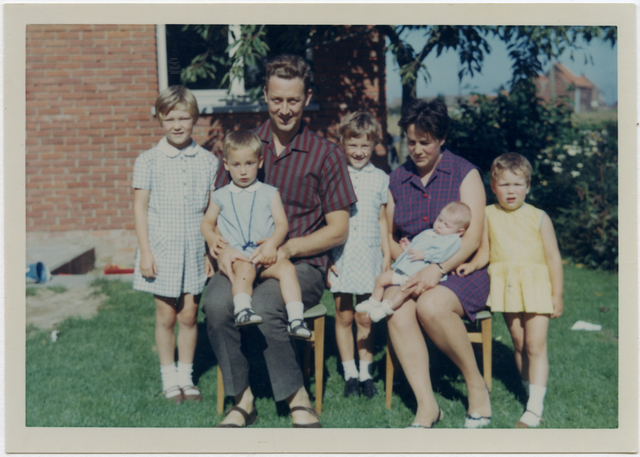
\includegraphics[width=\textwidth]{FO-60-01055.jpg}\hfill
    \\[\smallskipamount]
	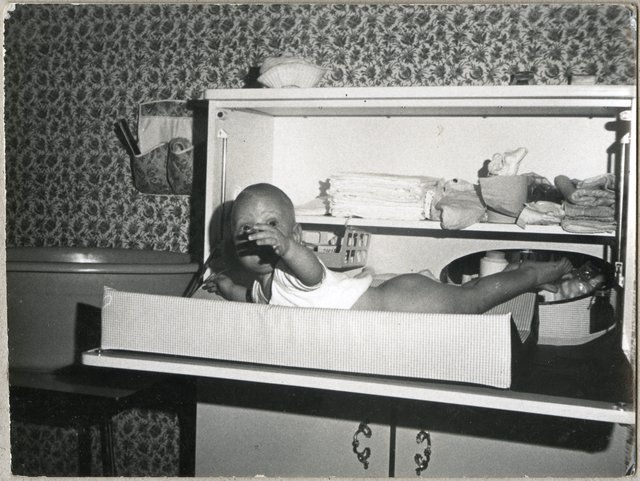
\includegraphics[width=\textwidth]{FO-70-00900.jpg}\hfill
	\caption[Best en slechtst scorende foto van thema geboorte]{een best scorende (boven) en slechtst scorende (onder) foto van het thema geboorte uit de fotocollectie van het Huis van Alijn.}
\end{figure}

De dertig meest voorkomende termen verwijzen naar mensen, kinderen en nakomelingen. Het model ziet ook enkele emoties in de beelden: liefde en affectie. Het merendeel van de foto’s waren ook portretten van moeder (en soms ook vader) met baby. Soms stonden er ook andere mensen, zoals broers, zussen, familieleden en vrienden op de foto. 

Uit de top 30 valt op dat er een groot verschil is tussen het aantal verschijningen van de meest voorkomende term (93 keer) en die op plaats 30 (7 keer). De top 11 komt in minstens de helft van de beelden voor. Het valt hierbij ook op dat term baby slechts aan de helft van de foto’s gegeven is.

Een opvallende vaststelling was dat het model de term \textit{dochter} niet kent; enkel \textit{zoon} werd gegeven. Doordat het voor ons niet mogelijk was om het verschil tussen een mannelijke en een vrouwelijke baby te zien, hebben we dit altijd als correct beschouwd.

Het model vergiste zich soms ook. Man en vrouw met kind werden in zestien van de gevallen door het model als een trouwfoto beschouwd. Ook de tags bruidegom (3 keer) en bruid kwamen voor (2 keer). Dit is vermoedelijk doordat op die foto’s de baby gewikkeld was in een sluier, wat verkeerdelijk door het model als een bruidssluier gepercipieerd werd.

\subsection{Huwelijk}
Voor dit thema waren vierhonderd beelden beschikbaar. Het general model van Clarifai scoorde erg goed op dit thema. Er werden 158 unieke termen gebruikt om de beelden te beschrijven. Gemiddeld waren 15,2 tags correct, wat ruim boven het gemiddelde is van alle beelden. Het maximale aantal correcte tags was twintig, het minste acht. Slechts zeven beelden hadden minder dan tien correcte tags, wat maar 1,75\% van het totaal aantal trouwfoto’s is!

\begin{figure}
	\centering
	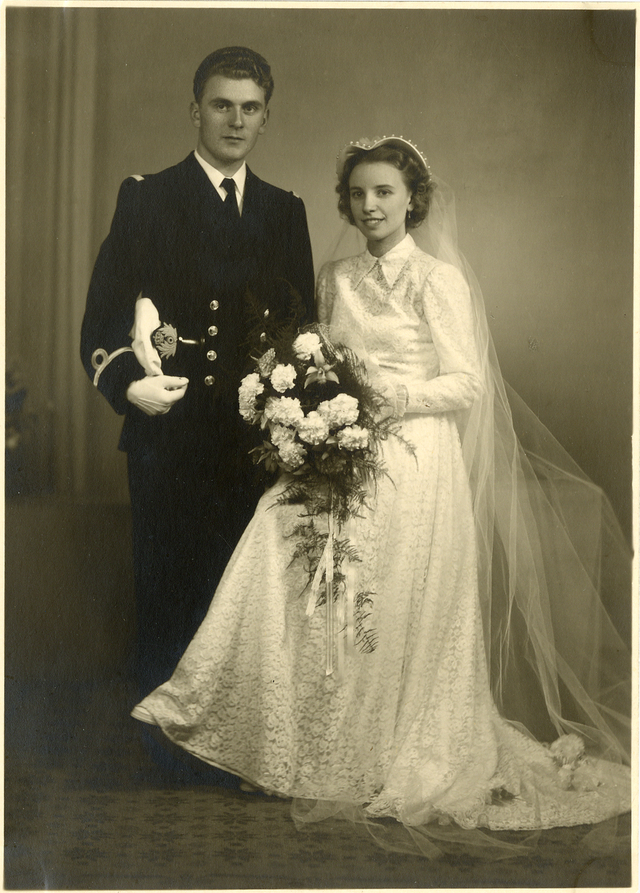
\includegraphics[width=0.505\textwidth]{FO-40-00650.jpg}\hfill
	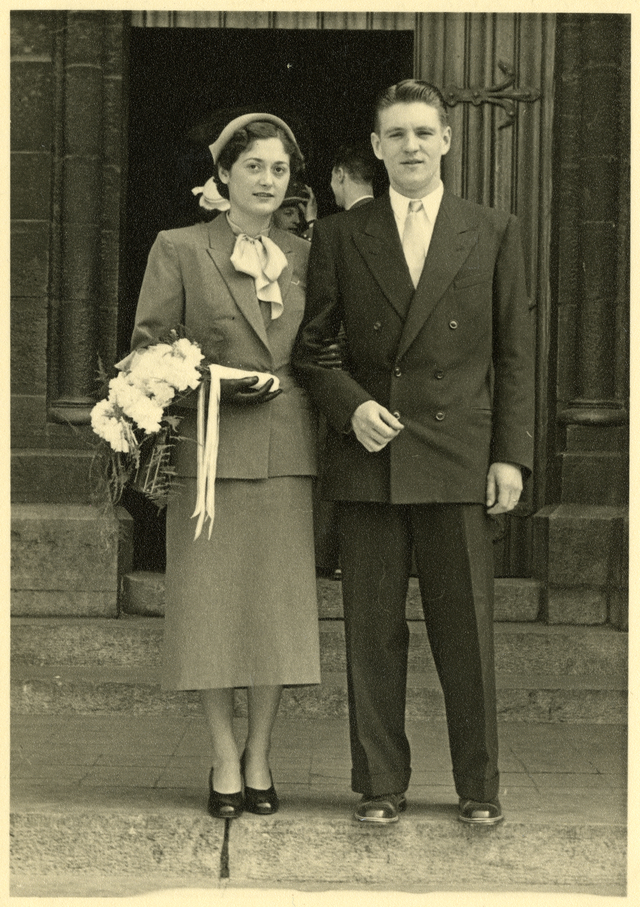
\includegraphics[width=0.495\textwidth]{FO-50-01313.jpg}\hfill
	\caption[Best en slechtst scorende foto van thema huwelijk]{een best scorende (links) en slechtst scorende (rechts) foto van het thema huwelijk uit de fotocollectie van het Huis van Alijn.}
\end{figure}

De dertig meest voorkomende termen verwijzen naar termen die je verwacht bij trouwfoto’s: mensen, een koppel, vrouw, man, bruid, bruidegom, boeket, op een bruiloft, in smoking en (trouw)jurk. Ook in deze foto’s wordt liefde gezien. 

De top tien van de termen komt in minstens de helft van de beelden voor. We stellen hier tevens een verschil vast tussen de meest (399 keer) en minst (48 keer) voorkomende term. Het valt op dat de term bruiloft 341 keer voorkomt; die van huwelijk 72 keer.

\begin{table}
	\centering
	\begin{tabular}{*{3}{l}}
		mensen (399) & sluier (198) & verschillende (83) \\
		vrouw (387) & groep (160) & smoking (75) \\
		volwassene (377) & jurk (159) & huwelijk (72) \\
		man (354) & ceremonie (147) & bruids (63) \\
		bruiloft (341) & gezichtsexpressie (132) & veel (58) \\
		portret (316) & samenkomen (127) & verbintenis (57) \\
		kledij (311) & liefde (121) & meisje (56) \\
		bruidegom (255) & monochroom (117) & koppel (55) \\
		twee (251) & bloemstuk (101) & kind (53) \\
		bruid (239) & familie (99) & boeket (48) \\	
	\end{tabular}
	\caption{De dertig meest voorkomende tags van trouwfoto's met het ingebouwde Clarifai-model}
	\label{tab:30-termen-huwelijk}
\end{table}

Uit analyse van de termen kan geconcludeerd worden dat het ingebouwde model van de Clarifai API trouwfoto’s kan onderscheiden zonder dat verdere training nodig is.

\subsection{Sinterklaas}

Zoals verwacht scoorde het Clarifai model niet goed op het taggen van de foto’s over Sinterklaas. Voor dit thema waren 97 beelden beschikbaar. Er werden slechts 51 unieke termen gebruikt om de beelden te beschrijven. Dit is 70 termen minder dan geboorte, dat na Sinterklaas de minst unieke termen heeft. Gemiddeld waren slechts tien tags correct, wat ruim onder het gemiddelde is van alle beelden (13,6). Het maximale aantal correcte tags was vijftien, het minste zeven. 48 beelden hadden minder dan tien correcte tags, wat 49,5\% van het totaal aantal Sinterklaasfoto’s is.

\begin{figure}
	\centering
	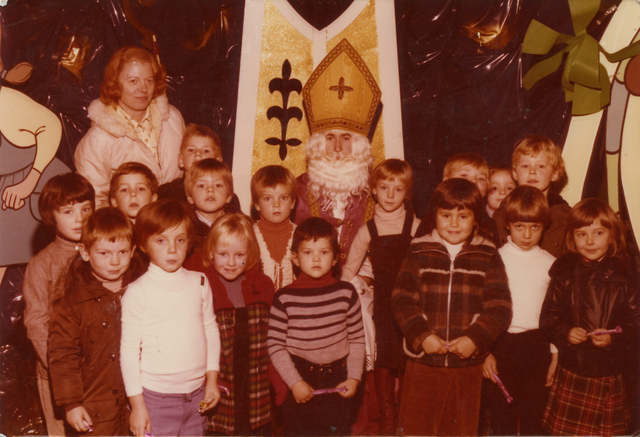
\includegraphics[width=0.67\textwidth]{FO-70-00254.jpg}\hfill
	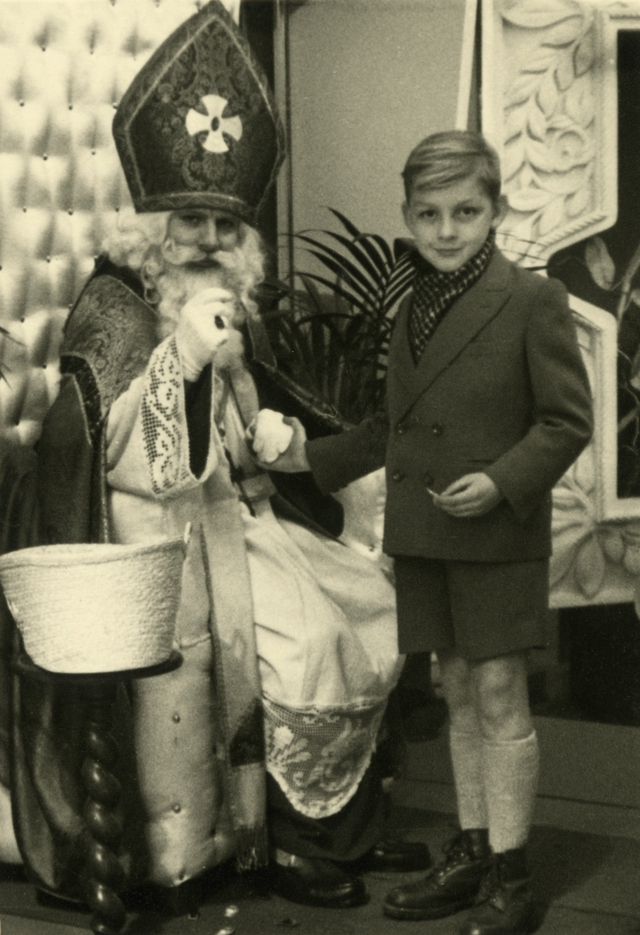
\includegraphics[width=0.32\textwidth]{FO-50-00439.jpg}\hfill
	\caption[Best en slechtst scorende foto van thema Sinterklaas]{een best scorende (links) en slechtst scorende (rechts) foto van het thema Sinterklaas uit de fotocollectie van het Huis van Alijn.}
\end{figure}

De reden voor deze lage cijfers komt zeer waarschijnlijk doordat het model de concepten van Sinterklaas niet kent. Het model gaf zeer regelmatig de tag \textit{retro} bij deze beelden, maar die werd steeds als incorrect aangevinkt. Alle beelden van Huis van Alijn zijn immers retro als het met hedendaagse ogen bekeken wordt. Daarnaast werden ook de termen \textit{zoon}, \textit{nakomelingen} en \textit{familie} als incorrect gevalideerd als er geen ouder of volwassene op de foto staat. 

De dertig meest voorkomende tags verwijzen naar een portret van twee, drie of vier mensen met volwassene(n) en kind(eren). De 97 beelden waren ook portretten van een of meerdere kinderen, soms vergezeld van volwassenen, met Sinterklaas. Wat opvalt is dat de tags sterk de nadruk op kleding leggen: kledij, sluier, outfit, kostuum, toga, bovenkleding. 

Ook bij deze beelden is er een groot verschil tussen de meest voorkomende termen en de minst voorkomende termen. Mensen en kledij komen in alle foto’s voor, terwijl meisje, toga en zitten voor slechts vijf foto’s gebruikt werden. De top 7 van de tags werd aan minstens de helft van de beelden gegeven. 

\begin{table}
	\centering
	\begin{tabular}{*{3}{l}}
		mensen (97) & drie (24) & broer of zus (10) \\
		kledij (97) & gezichtsexpressie (21) & vier (8) \\
		volwassene (95) & samenkomen (20) & bovenkleding (7) \\
		portret (91) & groep (19) & recreatie (7) \\
		kind (90) & kostuum (15) & acteur (6) \\
		man (86) & verschillende (15) & sepia (6) \\
		twee (53) & jongen (14) & uniform (6) \\
		monochroom (30) & vrouw (14) & meisje (5) \\
		outfit (30) & familie (13) & toga (5) \\
		sluier (25) & jas (10) & zitten (5) \\
	\end{tabular}
	\caption{De dertig meest voorkomende tags van Sinterklaasfoto's met het ingebouwde Clarifai-model}
	\label{tab:30-termen-sint}
\end{table}

\subsection{Speelgoed}

Er waren 101 foto’s voor dit thema. Net als bij Sinterklaas presteert Clarifai voor deze foto’s onder het gemiddelde. Gemiddeld waren 11,3 tags correct en hadden 23 beelden minder dan tien correcte tags (22,8\%). De slechts scorende foto had 6 juiste tags; voor de best scorende foto’s waren dit 17 tags. Voor het beschrijven van deze foto’s werden 126 unieke termen gebruikt.

\begin{figure}
	\centering
	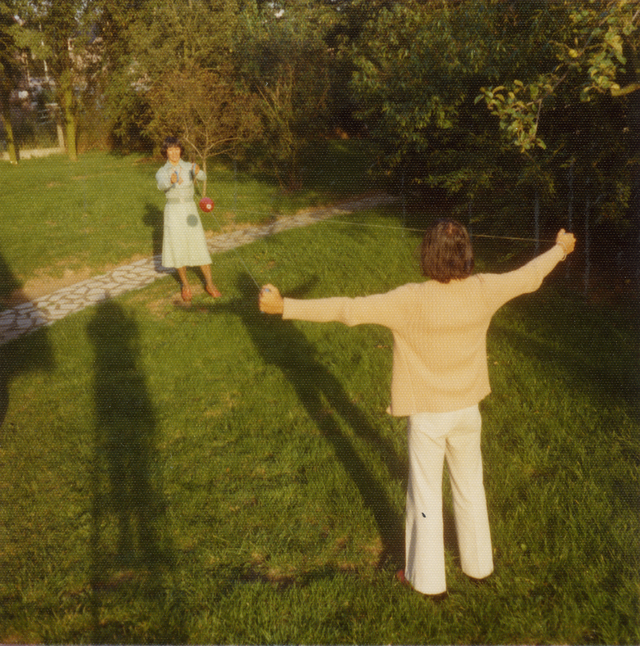
\includegraphics[width=0.495\textwidth]{FO-70-00621.jpg}\hfill
	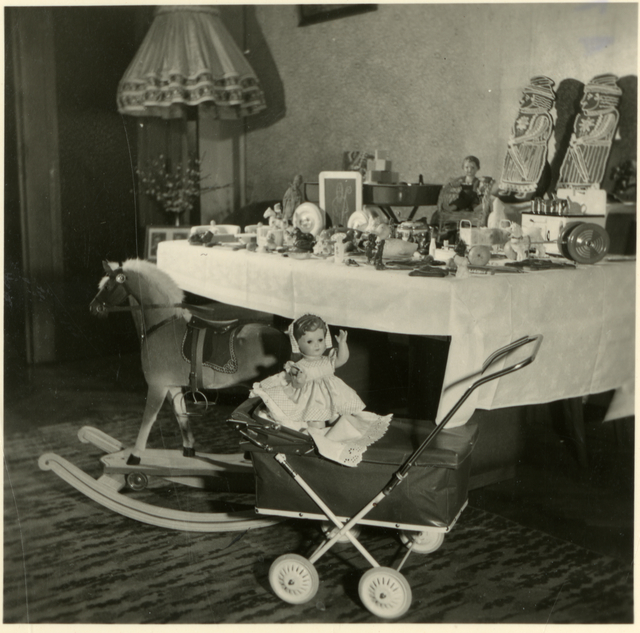
\includegraphics[width=0.495\textwidth]{FO-50-02073.jpg}\hfill
	\caption[Best en slechtst scorende foto van thema speelgoed]{een best scorende (links) en slechtst scorende (rechts) foto van het thema speelgoed uit de fotocollectie van het Huis van Alijn.}
\end{figure}

De dertig meest voorkomende termen verwijzen vooral naar kinderen, slechts in mindere mate naar speelgoed zelf. Het valt bijvoorbeeld op dat het afgebeelde speelgoed vaak niet herkend (of getagged) werd. Wel wordt er plezier en recreatie herkend. De term speelgoed (18 keer) komt ook voor, maar wel in mindere mate, net als vrije tijd (5 keer), spelen (5 keer) en spel (4 keer). Het ingebouwde model is bijgevolg niet voldoende om het merendeel van de speelgoedfoto’s eruit te halen.

De grote verschillen tussen de meest (100 keer) en minst (9 keer) voorkomende termen vallen op. Enkel de top 4 van de termen wordt aan minstens de helft van de beelden gegeven. Dit komt vermoedelijk omdat deze foto’s een minder vast format hadden dan de foto’s van de vorige thema’s. Die foto’s waren vaak portretten van resp. moeders/ouders met hun pasgeboren kind, bruid en bruidegom op hun trouw en kinderen met Sinterklaas. De speelgoedfoto’s hadden een grotere variëteit aan composities: portretten van kinderen die met hun speelgoed poseerden, maar ook kinderen en/of volwassenen die gezamenlijk een spel speelden. 

\begin{table}
	\centering
	\begin{tabular}{*{3}{l}}
		mensen (100) & recreatie (29) & speelgoed (18) \\
		kind (96) & twee (29) & broer of zus (17) \\
		kledij (65) & binnenshuis (28) & straat (17) \\
		portret (51) & familie (25) & voertuig (17) \\
		kamer (48) & groep (25) & thuis (16) \\
		jongen (44) & volwassene (22) & vrouw (14) \\
		monochroom (43) & zitten (22) & sepia (12) \\
		meisje (42) & samenkomen (20) & zitplaats (11) \\
		meubels (38) & gezichtsexpressie (18) & stoel (10) \\
		één (34) & plezier (18) & man (9) \\
	\end{tabular}
	\caption{De dertig meest voorkomende tags van de speelgoedfoto's met het ingebouwde Clarifai-model}
	\label{tab:30-termen-speelgoed}
\end{table}

Naar de reden voor de mindere score voor deze beelden is het gissen. Net zoals bij Sinterklaas werden vaak de termen \textit{retro} of \textit{vintage} gegeven, wat als fout beschouwd werd. Idem voor de termen \textit{zoon}, \textit{nakomelingen} of \textit{familie}, wanneer er geen ouder op de foto staat. Ook vergiste het model zich regelmatig. Kinderen werden vaak als volwassene getagged of kregen een fout gender (bv. een jongen die als meisje gezien werd). Poppen werden dan weer vaak als baby gelabeld. Het valt op dat de tags zich hoofdzakelijk op mensen concentreren. Mogelijk is het model minder goed in objectherkenning, maar dit moet verder onderzocht worden.

\subsection{Vakantie}

Het ingebouwde model van Clarifai scoorde goed op de 151 vakantiefoto’s, in lijn met het algemene gemiddelde.  Er werden 212 unieke termen gebruikt om de beelden te beschrijven. Gemiddeld waren 13,4 tags correct. Het maximale aantal correcte tags was twintig, het minste negen. Slechts twaalf beelden hadden minder dan tien correcte tags (8\%).

\begin{figure}
	\centering
	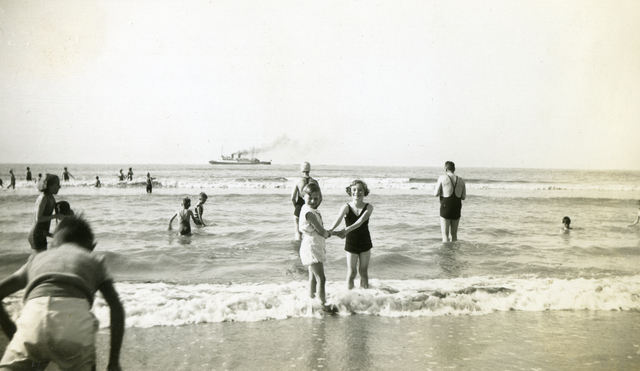
\includegraphics[width=\textwidth]{FO-30-00319_a3.jpg}\hfill
	\\[\smallskipamount]
	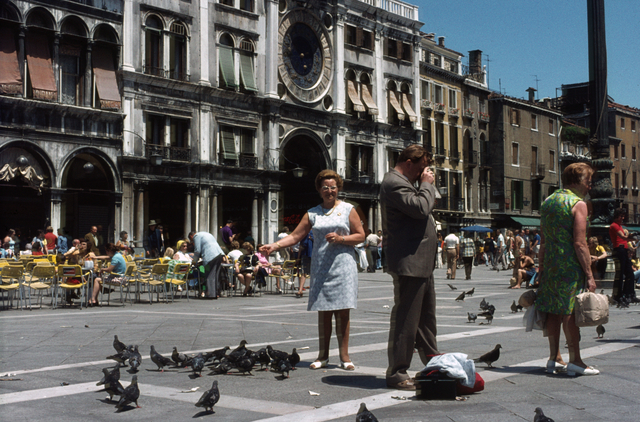
\includegraphics[width=\textwidth]{DIA-0006-0135.jpg}\hfill
	\caption[Best en slechtst scorende foto van thema vakantie]{een best scorende (boven) en slechtst scorende (onder) foto van het thema vakantie uit de fotocollectie van het Huis van Alijn.}
\end{figure}

De dertig meest voorkomende termen verwijzen naar mensen, vrije tijd, onderweg zijn en het strand. Het model ziet ook plezier in de beelden. Eveneens wordt het thema vakantie in negentien foto’s herkend, net zoals toerist (13 keer) en toerisme (8 keer).

Ook deze foto’s hebben geen vast format. Het zijn vakantiekiekjes. Dit verklaart de grote verscheidenheid aan termen om de beelden te beschrijven. De top 7 van de termen komt in minstens de helft van de beelden voor. Zoals bij de andere thema’s is er een groot verschil tussen het aantal verschijningen van de meest voorkomende term (142 keer) en de minst voorkomende term (17 keer). 

\begin{table}
	\centering
	\begin{tabular}{*{3}{l}}
		mensen (142) & straat (47) & meisje (23) \\
		volwassene (115) & voertuig (46) & weg (23) \\
		vrouw (98) & portret (35) & landschap (21) \\
		man (83) & veel (32) & water (21) \\
		recreatie (81) & strand (30) & vrije tijd (20) \\
		reizen (79) & monochroom (30) & vakantie (19) \\
		kledij (77) & buitenshuis (30) & familie (18) \\
		groep (75) & verschillende (30) & plezier (18) \\
		kind (50) & stad (26) & kust (18) \\
		samenkomen (48) & twee (25) & gebouw (17) \\
	\end{tabular}
	\caption{De dertig meest voorkomende tags van de vakantiefoto's met het ingebouwde Clarifai-model}
	\label{tab:30-termen-vakantie}
\end{table}

\section{Toepassen in de praktijk?}

Het loslaten van het ingebouwde model van Clarifai op de 845 beelden van Huis van Alijn leverde 11.517 juiste (68,15\%) en 5.383 foute (31,85\%) tags op. Dit gebeurde in ongeveer 35 minuten. Om dit in een productieomgeving te gebruiken, zijn een aantal strategieën mogelijk om het aantal fouten te verkleinen.

\subsection{Instellen van een drempelwaarde}

Er kan een drempelwaarde ingesteld worden om het aantal foute tags te verkleinen. Bij het instellen van een drempelwaarde worden alleen maar tags aanvaard waarvan de waarschijnlijkheidsscore groter is dan de drempelwaarde. Bij het uitvoeren van de case werd geen drempelwaarde ingesteld. De hoogste waarschijnlijkheidsscore van een correcte tag was 100\%, de laagste 64,7\%.

Indien het museum de drempelwaarde instelt op 90\%, krijgt het 82\% van het totaal aantal juiste tags. 25\% van de verkregen tags zijn dan fout. De drempelwaarde kan nog hoger gesteld worden, op 95\%, maar dan krijgt het slechts 55\% van het totaal aantal juiste tags. Slechts 17\% van de verkregen tags zijn dan verkeerd. De drempelwaarde kan verlaagd worden naar 85\% om een groter aandeel van de juiste tags te hebben, maar dan zijn 29,6\% van het aantal tags fout. Nu is dit aantal 31,85\% zonder drempelwaarde (tabel \ref{tab:instellen-drempelwaarde}).

\begin{table}
    \centering
	\begin{tabular}{*{3}{c}}
		\toprule
		drempelwaarde (\%) & aandeel juiste tags (\%) & $\sharp$ foute tags (\%) \\
        \midrule
		95 & 55 & 17 \\
        [\smallskipamount]
		90 & 85 & 25 \\
        [\smallskipamount]
		85 & 94,8 & 29,6 \\
        [\smallskipamount]
		geen & 100 & 31,85 \\
		\bottomrule
	\end{tabular}
	\caption{Verhouding tussen drempelwaarde, totaal aantal van de juiste tags en het aantal foute tags}
	\label{tab:instellen-drempelwaarde}
\end{table}

\subsection{Selectie maken van thema’s}

Een andere strategie om fouten te verkleinen is om een selectie te maken van de foto’s die door de CV API gelabeld moeten worden. Het museum zou ervoor kunnen kiezen om thema’s waarmee het ingebouwde model niet vertrouwd is, niet te laten labelen, zoals bijvoorbeeld de Sinterklaasfoto’s. Deze foto’s doen immers het gemiddelde dalen en het aantal foute tags stijgen. Een nadeel aan deze strategie is dat de foto’s al op voorhand ingedeeld moeten zijn in thema’s.
\chapter{Resultaten met de custom  modellen}
\label{ch:resultaten-custom-model}

In ongeveer een kwartier tijd hebben zowel het periodemodel als het themamodel de 845 beelden van Huis van Alijn gelabeld met periodes of thema’s. In die 845 beelden zitten ook de beelden die gebruikt werden voor training en validatie. Het is opmerkelijk om vast te stellen dat ook beelden die als trainingsbeeld ingegeven werden, soms door de modellen fout geclassificeerd worden.

In dit hoofdstuk worden afzonderlijk de resultaten van beide modellen besproken. Tot slot zal net als in hoofdstuk \ref{ch:resultaten-ingebouwd-model} suggesties gedaan worden voor de toepassing van de modellen in de praktijk.
    
Net zoals het ingebouwde model uit het vorige hoofdstuk, geven de custom modellen meerdere tags per foto. Omdat een foto slechts ingedeeld kan worden in één thema, houden we enkel rekening met de tag die de hoogste waarschijnlijkheiddscore gekregen heeft. 

\section{Themamodel}
\label{sec:themamodel}

Het Themamodel heeft 845 beelden geanalyseerd en geclassificeerd. 753 beelden (89\%) werden correct geclassificeerd.  De waarschijnlijkheidsscore van de tags bevond zich tussen 100\% en 39\% en had een gemiddelde van 94,6\%. De gemiddelde rappel voor de vijf thema’s is 90\%, terwijl de gemiddelde precisie een waarde van 86\% heeft.

\begin{table}
	\centering
     \renewcommand\arraystretch{1.2}
    \begin{tabular}{l|ccc|rrr}
        \toprule
         & true positives  & false negatives & false positives & rappel & precisie & \textit{F$_{1}$}-score \\
        \midrule
        geboorte & 81 & 15 & 50 & 84,4\% & 61,8\% & 71,4\% \\
        huwelijk & 346 & 54 & 6 & 86,5\% & 98,3\% & 92\% \\
        Sint & 93 & 4 & 1 & 95,9\% & 98,9\% & 97,4\% \\
        speelgoed & 88 & 13 & 21 & 87,1\% & 80,7\% & 83,8\% \\
        vakantie & 145 & 6 & 14 & 96\% & 91,2\% & 93,6\% \\
        \midrule
        gemiddelde & 150,6 & 18,4 & 18,4 & 90\% & 86,2\% & 87,6\% \\
        \bottomrule
    \end{tabular}
    \caption{De resultaten (rappel, precisie en \textit{F$_{1}$}-score) van het Themamodel op de volledige dataset van Huis van Alijn.}
    \label{tab:resultaten-themamodel}
\end{table}

Qua thema’s wordt de hoogste \textit{F$_{1}$}-score behaald bij het thema Sinterklaas (97\%). Dit thema haalde in hoofstuk \ref{ch:resultaten-ingebouwd-model} nog de slechtste resultaten, maar heeft in deze test de grootste precisie en de tweede grootste rappel. Dit is te verklaren doordat de foto’s sterk op elkaar lijken. Op iedere foto staat een oudere man met baard en mijter, vergezeld door een of meerdere kinderen die met de oude man op de foto poseren. Opvallend is ook de sterke score van de vakantiefoto’s (\textit{F$_{1}$}-score van 94\%), terwijl deze foto’s juist gekenmerkt worden door een grote variëteit (strandfoto’s, kampeerfoto’s, citytrips, wintersport,...).

De slechtste score wordt behaald met de geboortefoto’s. Vooral de precisie voor deze foto’s zijn ondermaats (62\%). Dit thema heeft 50 false positives\footnote{Dit zijn 50 foto's die foutief het label geboorte kregen.}. Veel huwelijksfoto’s (54 false negatives\footnote{~Dit zijn 54 huwelijksfoto's die niet als huwelijksfoto herkend werden.}) worden namelijk als geboortefoto herkend.  Net als in vorig hoofdstuk scoren de speelgoedfoto’s ook niet zo goed. Zowel de precisie als de rappel zijn lager dan het gemiddelde.

Sommige lagere scores zijn te wijten aan de vaag afgebakende thema’s door het museum. Sommige foto’s die door het museum ingedeeld werden in het thema speelgoed zijn  foto’s van kinderen met een stuk speelgoed op vakantie, terwijl er ook vakantiefoto’s zijn waar kinderen met speelgoed op poseren. Dit verklaart waarom het model zeven speelgoedfoto’s classificeert als vakantiefoto’s en vier vakantiefoto’s als speelgoedfoto’s. Het model heeft het ook moeilijk om poppen van baby’s te onderscheiden. Negen geboortefoto’s werden door het model ingedeeld in het thema speelgoed, terwijl zes speelgoedfoto’s als geboortefoto’s beschouwd werden (zie confusion matrix \ref{tab:confusion-matrix-themamodel}).

\begin{figure}
	\centering
	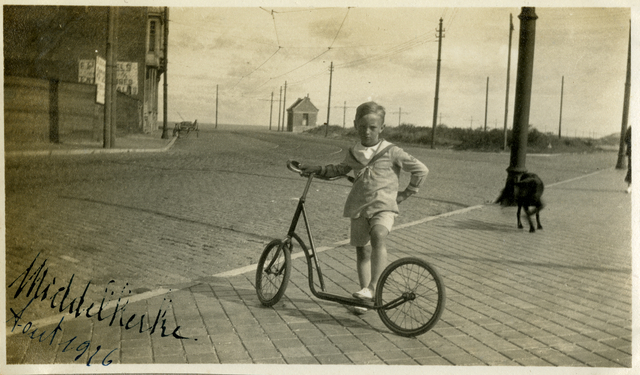
\includegraphics[width=\textwidth]{FO-20-00098.jpg}\hfill
	\\[\smallskipamount]
	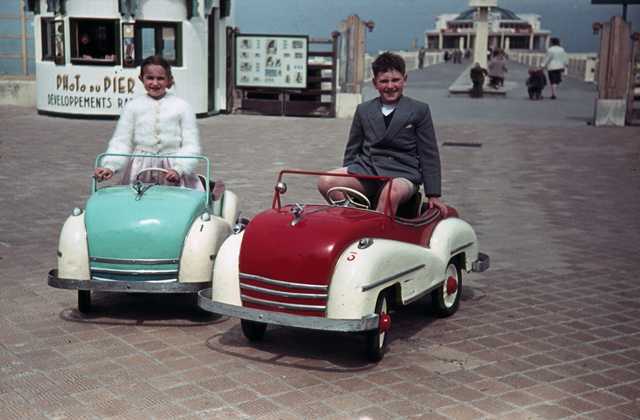
\includegraphics[width=\textwidth]{DIA-0037-0149.jpg}\hfill
	\caption[Voorbeeld van foto's van de thema's Vakantie en Speelgoed die gelijkend zijn]{Voorbeeld van foto's van de thema's Vakantie en Speelgoed die gelijkend zijn. De bovenste foto is een foto die door Huis van Alijn ingedeeld werd in het thema Speelgoed, de onderste foto is een vakantiefoto.}
\end{figure}

Net zoals in vorig hoofdstuk werd geanalyseerd of het model slecht scoort op foto’s uit bepaalde decennia. Dit lijkt niet het geval te zijn. Foto’s uit de jaren 60 (en 50) hebben een grotere foutenmarge, maar dit valt weer te verklaren door de grote hoeveelheid huwelijksfoto’s uit deze periode.

\begin{table}
    \centering
    \renewcommand\arraystretch{1.2}
    \settowidth\rotheadsize{\theadfont Feitelijk thema}   
    \begin{tabular}{@{} cc | cccccc}
        \toprule
        &  & & \multicolumn{5}{c}{\textbf{Voorspeld thema}}  \\
        &  & & geboorte & huwelijk & sint & speelgoed &  vakantie  \\
        \midrule
        \multirow{5}{*}[1ex]{\rothead {\textbf{Feitelijk thema}}}
        & geboorte   &  &  \cellcolor{hgpink}81 & 3 & 1 & 9 & 2 \\
        & huwelijk  &   & 43 & \cellcolor{hgpink}346 & 0 & 6 & 5 \\
        & sint  &   & 1 & 1 & \cellcolor{hgpink}93 & 2 & 0 \\
        & speelgoed  &  & 6 & 0 & 0 & \cellcolor{hgpink}88 & 7 \\
        & vakantie & & 0 & 2 & 0 & 4 & \cellcolor{hgpink}145 \\
        \bottomrule
    \end{tabular}
    \caption{Confusion matrix voor het Themamodel}
    \label{tab:confusion-matrix-themamodel}
\end{table}

\section{Periodemodel}
\label{sec:periodemodel}

Ook het Periodemodel heeft 845 beelden geanalyseerd en geclassificeerd. Omdat van 42 beelden de periode niet gekend was door het museum en we dus niet konden nagaan of het model ze juist geclassificeerd heeft, werden deze beelden niet meegerekend bij de beoordeling van de resultaten. 

Het model had 460 beelden (57\%) correct geclassificeerd. De waarschijnlijkheidsscore van de tags bevond zich tussen 94\% en 20\% en had een gemiddelde van slechts 55\%. Dit kan betekenen dat het model ofwel te weinig trainingsbeelden had om de verschillende concepten te kunnen onderscheiden, of dat de taak te moeilijk is voor een CV API. De gemiddelde rappel voor de tien periodes is maar 57\%, terwijl de gemiddelde precisie een waarde van 62\% heeft.

\begin{table}
	\centering
    \renewcommand\arraystretch{1.2}
    \begin{tabular}{l|ccc|rrr}
        \toprule
        & true positives  & false negatives & false positives & rappel & precisie & \textit{F$_{1}$}-score \\ 
        \midrule
        00s & 3 & 6 & 0 & 33,3\% & 100\% & 50\% \\ 
        10s & 13 & 3 & 8 &  81,3\% & 61,9\% & 70,3\% \\ 
        20s & 14 & 18 & 15 & 43,8\% & 48,3\% & 45,9\% \\ 
        30s & 34 & 20 & 45  & 63\% & 43\% & 51,1\% \\ 
        40s & 40 & 21 & 70  & 65,6\% & 36,4\% & 46,8\% \\ 
        50s & 110 & 99 & 71  & 52,6\% & 60,8\% & 56,4\% \\ 
        60s & 120 & 106 & 56  & 53,1\% & 68,2\% & 59,7\% \\ 
        70s & 73 & 41 & 51  & 64\% & 58,9\% & 61,3\% \\ 
        80s & 43 & 18 & 24  & 70,5\% & 64,2\% & 67,2\% \\ 
        90s & 10 & 11 & 3  & 47,6\% & 77\% & 58,8\% \\ 
        \midrule
        gemiddelde & 46 & 34,3 & 34,3  & 57,5\% & 61,9\% & 56,7\% \\ 
        \bottomrule
    \end{tabular} 
    \caption{De resultaten (rappel, precisie en \textit{F$_{1}$}-score) van het Periodemodel op de volledige dataset van Huis van Alijn.}
    \label{tab:resultaten-periodemodel}
\end{table}

De hoogste F-score wordt behaald bij foto’s van de jaren 10 (70\%). Dit is nochtans een van de periodes met het laagst aantal trainingsbeelden (8 beelden). Vooral de rappel voor deze periode is erg goed (81\%). Ook de 80s scoren goed met een F-score van 67\%. Over het algemeen scoren de periodes vanaf de jaren 60 het best, waarbij de jaren 10 de uitzondering is. Misschien zijn zwart-wit foto’s uit de jaren 20 tot en met 60 vergelijkbaar qua kleur?

De slechtste scores worden behaald met foto’s uit de jaren 20 en 40, met een respectievelijke F-score van 46\% en 47\%. Bij de jaren 40 is de rappel goed (66\%), maar is de precisie erg laag (36\%). Het heeft namelijk 70 false positives. Dit komt doordat veel foto’s uit de jaren 50 (43 foto’s), en in mindere mate jaren 60 (13 foto’s) en 30 (9 foto’s), herkend wordt als een foto uit de jaren 40. Als het model fout is, dan vergist het zich meestal met de omliggende periodes (zie confustion matrix \ref{tab:confusion-matrix-periodemodel}).

\begin{table}
    \centering
    \renewcommand\arraystretch{1.2}
    \settowidth\rotheadsize{\theadfont Feitelijk thema}
    
    \begin{tabular}{@{} cc | ccccccccccc}
        \toprule
        &  & & \multicolumn{10}{c}{\textbf{Voorspelde periode}}  \\
        &  & & 00s & 10s & 20s & 30s & 40s & 50s & 60s & 70s & 80s & 90s \\
        \midrule
        \multirow{10}{*}[1ex]{\rothead {\textbf{Feitelijke periode}}}
        & 00s   &  & \cellcolor{hgpink}3 & 2 & 1 & 0 & \cellcolor{hgpink}3 & 0 & 0 & 0 & 0 & 0 \\
        & 10s  &   & 0 & \cellcolor{hgpink}13 & 1 & 1 & 1 & 0 & 0 & 0 & 0 & 0 \\
        & 20s  &   & 0 & 2 & \cellcolor{hgpink}14 & \cellcolor{hgpink}12 & 0 & 3 & 0 & 0 & 0 & 0 \\
        & 30s  &  & 0 & 0 & 4 & \cellcolor{hgpink}34 & 9 & 4 & 3 & 0 & 0 & 0 \\
        & 40s & & 0 & 1 & 2 & 4 & \cellcolor{hgpink}40 & 13 & 0 & 0 & 0 & 0 \\
        & 50s   &  & 0 & 3 & 3 & 15 & 43 & \cellcolor{hgpink}110 & 32 & 3 &0 & 0 \\
        & 60s  &   & 0 & 0 & 3 & 8 & 13 & 42 & \cellcolor{hgpink}120 & 31 & 9 & 0 \\
        & 70s  &   & 0 & 0 & 1 & 3 & 0 & 9 & 19 & \cellcolor{hgpink}73 & 8 & 1 \\
        & 80s  &  & 0 & 0 & 0 & 0 & 0 & 0 & 2 & 14 & \cellcolor{hgpink}43 & 2 \\
        & 90s & & 0 & 0 & 0 & 1 & 0 & 0 & 0 & 3 & \cellcolor{hgpink}7 & \cellcolor{hgpink}10 \\
        \bottomrule
    \end{tabular}
    \caption{Confusion matrix voor het Periodemodel}
    \label{tab:confusion-matrix-periodemodel}
\end{table}

Twee periodes behalen een lage rappel, maar een erg hoge precisie. Foto’s uit de jaren 00 hebben een rappel van slechts 33\%, maar een precisie van 100\%; voor de jaren 90 gaat het om een rappel van 48\% en een precisie van 77\%. Deze periodes scoorden tevens minder goed in de validatieset en behoren tot de groep met het minst aantal trainingsbeelden (respectievelijk vier en tien beelden). 

\section{Toepassen in de praktijk?}
\label{sec:custom-toepassen-praktijk}
Het Periodemodel is niet voldoende performant om in de praktijk toe te passen. De foutenpercentage is te hoog en de waarschijnlijkheidsscores zijn te laag om goede conclusies te kunnen trekken. In deze sectie wordt daarom enkel gefocust op het Themamodel.

Het is moeilijker dan in \ref{sec:ingebouwd-toepassen-praktijk} om duidelijke conclusies te trekken omdat we slechts 845 resultaten hebben om te beoordelen. Uit de resultaten lijkt dat een CV API vooral goed te trainen is op beelden die een duidelijke weergave en thematiek hebben, zoals de Sinterklaasfoto’s.

Wat betreft waarschijnlijkheidsscores en drempelwaarden zijn er twee strategieën die gevolgd kunnen worden: 
\begin{enumerate}
        \item instellen van een drempelwaarde;
        \item rekening houden met de waarschijnlijkheidsscore van de concept met de tweede hoogste score.
\end{enumerate}

\subsection{Instellen van een drempelwaarde}
Zoals reeds vermeld is de gemiddelde waarschijnlijkheidsscore 94,6\% voor zowel juist als foutief geklasseerde foto’s. De gemiddelde waarschijnlijkheidsscore voor de juiste classificaties ligt echter hoger (97\%), terwijl die voor de foute lager ligt (77\%). De mediaan\footnote{De mediaan is het midden van een verzameling van gegevens. 50\% heeft bijgevolg een waarde lager dan de mediaan; 50\% dan weer een waarde hoger dan de mediaan.} is respectievelijk 100\% en 80\%. Ook uit figuur \ref{fig:boxplot-tag1} valt duidelijk te zien dat het grootste aandeel van de waarschijnlijkheidsscores van de juiste tags buiten de grens van het grootste aandeel waarschijnlijkheidsscores van de foute tags ligt. Het is dus mogelijk om een drempelwaarde in te stellen om zoveel mogelijk juiste classificaties te behouden en foute classificaties te weren (zie tabel \ref{tab:drempelwaarde-custom-tag1}). 

\begin{figure}
	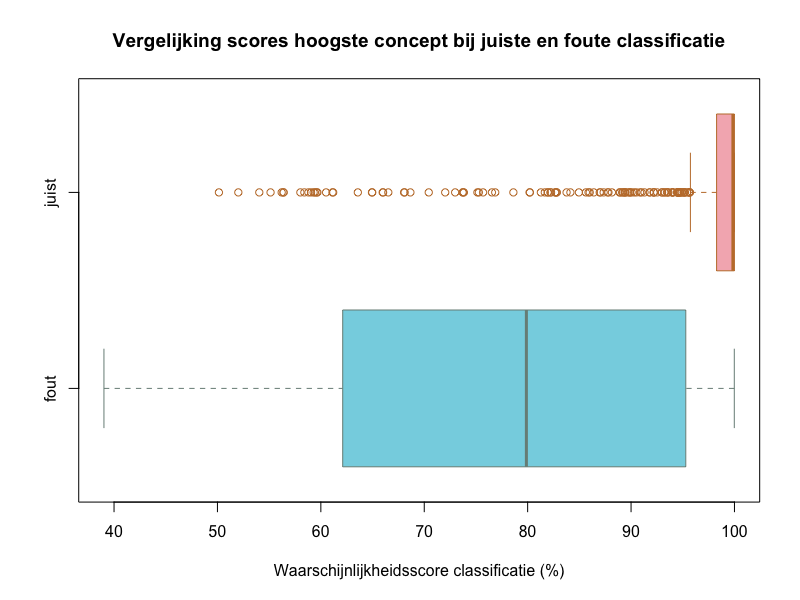
\includegraphics[width=\textwidth]
	{boxplot_hoogste_concept.png}
	\caption[Vergelijking van de waarschijnlijkheidsscores van de juiste en foute classicaties van het custom model]{Twee boxplots die de waarschijnlijkheidsscores vergelijken van het Periodemodel bij juiste en foute classificatie. In tegenstelling tot in figuur \ref{fig:boxplot-clarifai} is er geen overlap tussen de interkwartielafstand van de foute classificaties en de boxplot van de juiste classificaties.}
	\label{fig:boxplot-tag1}
\end{figure}

\begin{table}
	\renewcommand\arraystretch{1.2}
	\centering
	\begin{tabular}{*{3}{c}}
		\toprule
		drempelwaarde (\%) & aandeel juiste classificaties (\%) & aantal foute classificaties (\%) \\
		\midrule
		95 & 87 & 3,7 \\
		[\smallskipamount]
		90 & 91 & 4,6 \\
		[\smallskipamount]
		80 & 95 & 6,6 \\
		[\smallskipamount]
		55 & 100 & 11 \\
		\bottomrule
	\end{tabular}
	\caption{Verhouding tussen drempelwaarde, totaal aantal van de juiste classificaties en het aantal foute classificaties}
	\label{tab:drempelwaarde-custom-tag1}
\end{table}

\subsection{Rekening houden met de waarschijnlijkheidsscore van de tweede tag}
Anderzijds kan er ook gekeken worden naar de waarschijnlijkheidsscore van het tweede hoogste concept dat door het model gegeven wordt. Als het model een foto correct geclassificeerd heeft, dan krijgt het tweede concept in 64\% van de gevallen een waarschijnlijkheiddscore van (afgerond) 0\%. Wanneer het model een foto fout geclassificeerd heeft, dan ligt de mediaan van de waarschijlijkheidsscore voor het tweede concept op 17\% en het gemiddelde op 19\%. Ook uit figuur \ref{fig:boxplot-tag2} blijkt dat er weinig overlap is tussen de waarschijnlijkheidsscores van de tweede tag als de classificatie juist of fout is. Door de tags te weerhouden waarvan het tweede concept een te hoge score heeft, kunnen eveneens fouten vermeden worden. In tabel \ref{tab:drempelwaarde-custom-tag2} worden hiervoor ook enkele voorstellen gedaan.

\begin{figure}
	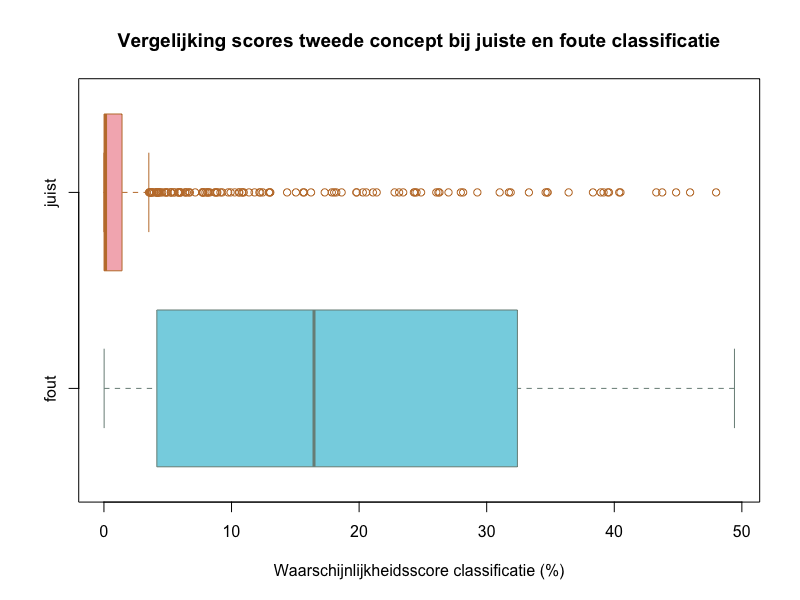
\includegraphics[width=\textwidth]
	{boxplot_tweede_concept.png}
	\caption[Vergelijking van de waarschijnlijkheidsscores van de juiste en foute classicaties van het custom model]{Twee boxplots die de waarschijnlijkheidsscores vergelijken van het tweede concept van het Periodemodel bij juiste en foute classificatie. Net als in figuur \ref{fig:boxplot-tag1} is er geen overlap tussen de interkwartielafstand van de boxplot van de foute classificatie en de boxplot van de juiste classificatie.}
	\label{fig:boxplot-tag2}
\end{figure}

\begin{table}
	\renewcommand\arraystretch{1.2}
	\centering
	\begin{tabular}{*{3}{c}}
		\toprule
		drempelwaarde (\%) & aandeel juiste classificaties (\%) & aantal foute classificaties (\%) \\
		\midrule
		5 & 87,5 & 3,3 \\
		[\smallskipamount]
		10 & 91 ,6& 4,5 \\
		[\smallskipamount]
		15 & 93,6 & 5,6 \\
		[\smallskipamount]
		48 & 100 & 12,1 \\
		\bottomrule
	\end{tabular}
	\caption{Verhouding tussen een drempelwaarde voor het tweede hoogste concept, totaal aandeel van de juiste tags en het aantal foute tags}
	\label{tab:drempelwaarde-custom-tag2}
\end{table}


%...

%%=============================================================================
%% Conclusie
%%=============================================================================

\chapter{Conclusie}
\label{ch:conclusie}

Met deze bachelorproef wilden we een bijdrage leveren aan het gebruik van Computer Vision API's voor cultureel erfgoed. Op 845 beelden van Huis van Alijn en met Clarifai als API werd onderzocht of CV API’s in staat zijn om cultureel-erfgoedcollecties inhoudelijk te beschrijven. Dit onderzoek ging een stap verder dan andere musea die reeds CV API uittestten door de CV API te trainen om classificatieproblemen van Huis van Alijn op te lossen.

Clarifai was eenvoudig in gebruik en kan volgens ons ook gebruikt worden door mensen zonder programmeerervaring. Alle mogelijkheden van de CV API, zoals het laten taggen van beelden of het trainen van een eigen model, zijn namelijk te gebruiken via de webinterface.

Clarifai is in staat om erfgoedcollecties algemeen te beschrijven; ongeveer 70\% van de aangeleverde tags waren correct. De CV API scoorde iets beter op recente foto’s, maar deed het niet veel slechter op de oude foto’s. Zoals ook \textcite{Vanstappen2019} vaststelde is het sterke punt de performantie: in ongeveer 35 minuten werden 845 beelden van twintig tags voorzien. De custom modellen deden er zelfs maar een kwartief over om de classificaties uit te voeren.

In vergelijking met de beschrijvingen van de registratoren van Huis van Alijn stelden we vast dat Clarifai meer trefwoorden per beeld geeft en bovendien vollediger is. Clarifai gaf bijvoorbeeld 255 keer correct de term bruidegom aan de beelden, terwijl de registratoren dit maar voor tien beelden gebruikt hebben. Bovendien gaf Clarifai een ander soort inhoudelijke beschrijving aan de beelden. We zagen regelmatig tags terugkeren die emoties (liefde, affectie), sfeer (plezier, vriendschap) of activiteiten (reizen, winkelen) verwoorden. Dat soort beschrijving ontbrak bij de registratoren. Nochtans kunnen deze termen de bezoeker nieuwe ervaringen aanbieden om de collectie te ontdekken.

Wanneer erfgoedinstellingen de ingebouwde modellen van een CV API willen gebruiken moeten ze rekening houden met het gegeven dat de meeste van deze modellen ontwikkeld zijn in de Verenigde Staten en een universeel karakter hebben. Beelden die een typisch lokale (hier: Vlaamse/Belgische) traditie voorstellen, kunnen daarom niet geschikt zijn om te laten taggen met de ingebouwde modellen. Dat werd vastgesteld met de Sinterklaasfoto’s waar Clarifai maar 51\% correcte tags kon geven. 

Voor het classificeren van de foto’s per thema volstond het ingebouwde model niet. Hiervoor moest een eigen model ontwikkeld worden. Ook voor het classificeren van de foto’s per decennia maakten we een eigen model. Een pijnpunt bij het trainen van de modellen was de kleine en ongelijke dataset. Zulke kleine en ongelijke datasets zijn echter doorgaans de realiteit in erfgoedcollecties. Bij het Themamodel slaagden we erin om iedere klasse evenwaardig te trainen; bij het Periodemodel lukte dit niet omdat er te weinig beelden voor sommige klassen waren.

Dat vertaalt zich ook in de resultaten. Voor het Themamodel werden 95\% van de beelden correct geclassificeerd; voor het Periodemodel ging het maar om 57\%. Er is verder onderzoek nodig om te zien of het Periodemodel kans op slagen heeft met een grotere trainingset. Voor het Themamodel zouden de resultaten beter zijn als het museum consequenter is in het classificeren van de foto’s. Vakantiefoto’s werden namelijk soms door het museum als speelgoedfoto geclassificeerd omdat er een kind met een stuk speelgoed op stond. De CV API is vooral goed in het trainen van concepten met een duidelijke weergave en thematiek.

Om het aantal fouten te vermijden wordt in deze paper voorgesteld om een drempelwaarde in te stellen. Het is aan de musea om te bepalen welke foutenmarge toelaatbaar is. Bij de zelfgecreëerde modellen werd steeds de versie van het model geselecteerd waarvan de $F_1$-score het hoogste is. Als precisie of rappel de doorslaggevende factor is, dan kan men best de versie kiezen waarvan respectievelijk de precisie of rappel het hoogste scoort.

Hoewel we kunnen concluderen dat CV API geschikt zijn om de case van Huis van Alijn uit te voeren, is het niet mogelijk om uitspraken te doen voor alle cultureel-erfgoedcollecties. Daarvoor is de dataset niet representatief genoeg. Er is verder onderzoek nodig met beelden van andere soorten erfgoedmateriaal, denk aan schilderijen, beeldhouwwerken en museumobjecten. Tevens zijn verschillende use cases niet gedekt. In dit onderzoek werd enkel onderzocht hoe CV API kunnen helpen bij het doorzoekbaar maken van omvangrijke collecties en bij het classificeren van beelden op basis van vooraf bepaalde klassen. Uitdagingen zoals pre-iconografische en iconografische beschrijving\footnote{~Iconografie houdt het beschrijven en bestuderen van onderwerpen uit de beeldende kunst in. Het is een onderdeel van kunstwetenschappen. Pre-iconografie is het beschrijven van objecten in een kunstwerk en gaat de iconografie vooraf.}, het herkennen van personen en locaties, objectregistratie en topic detection vragen verder onderzoek. Voor Huis van Alijn kan nog verder uitgezocht worden hoe tags van Clarifai gekoppeld kunnen worden aan de termenlijst van Huis van Alijn of thesauri zoals AAT\footnote{~De Art \& Architecture Thesaurus (AAT) is een thesaurus die gebruikt wordt voor het beschrijven van cultureel-erfgoedcollecties, zie \url{http://www.getty.edu/research/tools/vocabularies/aat/}.}.

%%=============================================================================
%% Bijlagen
%%=============================================================================

\appendix
\renewcommand{\chaptername}{Appendix}

%%---------- Onderzoeksvoorstel -----------------------------------------------

\chapter{Onderzoeksvoorstel}

Het onderwerp van deze bachelorproef is gebaseerd op een onderzoeksvoorstel dat vooraf werd beoordeeld door de promotor. Dat voorstel is opgenomen in deze bijlage.

% Verwijzing naar het bestand met de inhoud van het onderzoeksvoorstel
%---------- Inleiding ---------------------------------------------------------

\section{Introductie} % The \section*{} command stops section numbering
\label{sec:introductie}

De Vlaamse Overheid investeert in het Vlaamse cultureel erfgoed door collectiebeherende instellingen te ondersteunen en kwaliteitslabels uit te reiken. In ruil voor die steun verwacht de Vlaamse Overheid dat die instellingen een aantal taken uitvoeren, waaronder het registreren, inventariseren en metadateren van cultureel-erfgoedobjecten op een gestandaardiseerde manier, het onderzoeken (en faciliteren van onderzoek) en het presenteren van de collectie.~\autocites{AKE2014}{Gatz2016}

De collectiebeherende instellingen lijden aan een historische achterstand m.b.t. de registratie van de eigen collectie~\autocite{Gatz2016}. In 2018 werd daarom een nieuwe subsidielijn opgestart om de digitale collectieregistratie weg te werken. Deze subsidielijn werd opgestart vanuit de vaststelling dat de competenties en strategie{\"e}n ontbreken om een inhaalbeweging te realiseren~\autocite{JeugdMediaC2018a}.

In de bachelorproef willen we onderzoeken in welke mate Computer Vision API's (vanaf nu afgekort als CVA), zoals Google Cloud Vision\footnote{\url{https://cloud.google.com/vision/}} of Microsoft Computer Vision API\footnote{\url{https://azure.microsoft.com/nl-nl/services/cognitive-services/computer-vision/}}, ingezet kunnen worden om dit registratieproces te versnellen en als strategie gebruikt kunnen worden om een inhaalbeweging te realiseren. Momenteel gebeuren registraties door domeinexperten. Dit is tijdrovend werk. Met behulp van artifici{\"e}le intelligentie (AI) kan dit proces deels geautomatiseerd worden. Dit geeft de collectieregistrator de mogelijkheid om zich met minder basaal werk bezig te houden en geeft de musea de kans hun collectie sneller te ontsluiten.

Het VKC Datahub Dashboard\footnote{\url{https://dashboard.vlaamsekunstcollectie.be}} geeft een goed beeld van de registratieachterstand in Vlaanderen. Dit dashboard analyseert de collectieregistratie van de Vlaamse musea voor Schone (en in de toekomst ook Hedendaagse) Kunsten die aangesloten zijn bij de VlaamseKunstCollectie (VKC)\footnote{\url{http://vlaamsekunstcollectie.be/}}, waaronder het aantal records ingevuld volgens de minimale registratie en het aantal records ingevuld volgens de basisregistratie.\footnote{De minimale registratie omvat de elementen en velden die in overeenstemming met de ICOM Code of Ethics minimaal gedocumenteerd moeten worden wanneer een object een museum binnenkomt: d.i. bewaarinstelling, objectnummer, titel, korte beschrijving, objectnaam, verwervingsmethode, verwervingsbron en verwervingsdatum. De velden voor de basisregistratie bevatten de acht velden voor minimale registratie en voegen hier nog een tiental andere velden aan toe. Voor meer info, zie het \href{https://www.projectcest.be/wiki/Publicatie:Invulboek_objecten/Profielen/Basisregistratie}{Invulboek Objecten op CEST}} Dit zijn cijfers van de grooste kunstmusea van Vlaanderen. Uit de cijfers blijkt dat vooral formele en administratieve gegevens geregistreerd worden; inhoudelijke informatie, zoals afgebeelde persoon of afgebeeld concept, die interessant is voor ontsluiting en onderzoek, ontbreekt hoofdzakelijk.

\begin{figure}[h]
	\caption{Het overzicht van de velden van de basisregistratie en het aantal keer dat ze aanwezig zijn in de collectiedata van MSK Gent.}
	\centering
	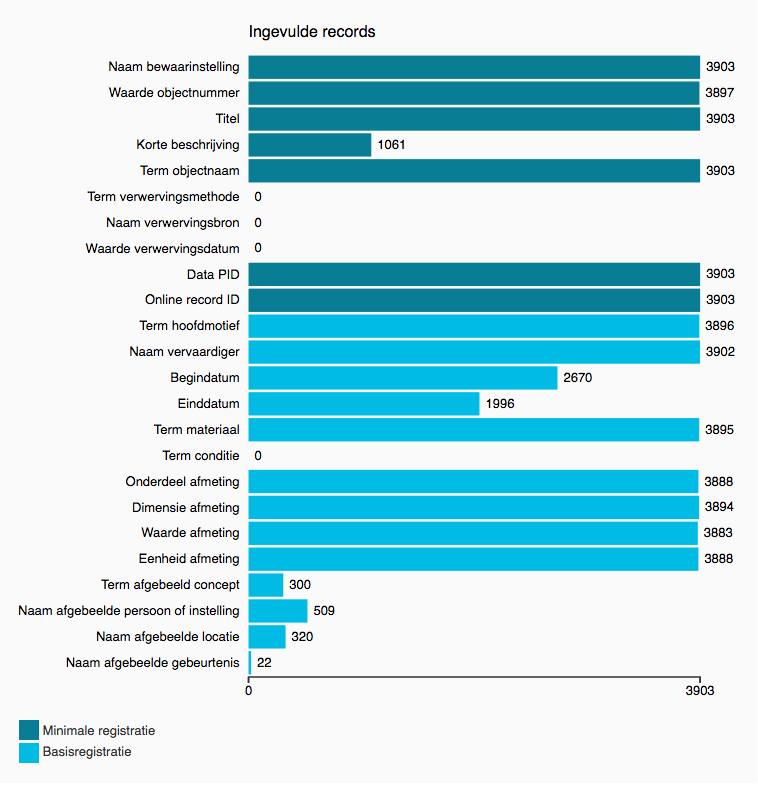
\includegraphics[width=\linewidth]{../voorstel/pictures/VKC_velden_basis.png}
\end{figure}

In het verleden werd reeds (theoretisch) onderzoek verricht naar het gebruik van Computer Vision voor cultureel erfgoed en kunst.\footnote{Zie infra, in het deel \emph{Stand van zaken}.} De resultaten van dit onderzoek waren veelbelovend. Nieuwe ontwikkelingen zorgen ervoor dat Computer Vision steeds meer accuraat wordt en steeds eenvoudiger in gebruik, waardoor het meer en meer een instrument wordt waarmee ook developers aan de slag kunnen~\autocite{Hindle2017}.

%---------- Stand van zaken ---------------------------------------------------

\section{Stand van zaken}
\label{sec:state-of-the-art}

\subsection{Computer Vision en (cultureel) erfgoed}
Een aantal instellingen maken al gebruik van Computer Vision voor de ontsluiting van hun collectie:
\begin{itemize}
	\item \textbf{The Museum of Modern Art (MoMA)}\footnote{\url{https://www.moma.org/}} gebruikte diensten van Google via \emph{Google Arts Culture Lab} om aan de historische foto's van afgelopen tentoonstellingen in MOMA foto's uit de kunstcollectie te koppelen. Het algoritme analyseerde hiervoor alle foto's van tentoonstellingszichten. Als het een kunstwerk op de foto's kon herkennen, dan werd er een koppeling gelegd met de afbeelding van dit kunstwerk in de collectie van MOMA.\footnote{Bekijk een voorbeeld over \href{https://www.moma.org/calendar/exhibitions/1767/installation_images/10473}{een tentoonstelling over C\`{e}zanne, Gaugain, Seurat en Van Gogh uit 1929}} MOMA stelde hierbij vast dat het logaritme vooral goed scoort op het vlak van tweedimensionele, statische afbeeldingen (bv. een afbeelding van een kunstwerk), maar dat het minder goede resultaten geeft met afbeeldingen van 3D-objecten (bv. een standbeeld) of bewegend beeld~\autocite{MOMA2018?}.

	\item Het \textbf{Smithsonian}\footnote{\url{https://www.smithsonianmag.com/}} gebruikt AI-technologie om stalen van planten te classificeren. Het Smithsonian is gestart met het systematisch digitaliseren van de collectie voor wetenschappers en in functie van online ontsluiting. De AI-technologie slaagde erin om via deze afbeeldingen twee gelijkaardige planten te onderscheiden met een succesgraad van meer dan 90\%~\autocite{Smith2017}.

	\item Het \textbf{Nasjonalmuseet}\footnote{\url{http://www.nasjonalmuseet.no/en/}} was het onderwerp van het \emph{Principal Components} onderzoek. Hierbij werd met het deep learning framework Caffe\footnote{Voor meer info, zie: \url{http://caffe.berkeleyvision.org/}} gezocht naar compositionele gelijkenissen tussen kunstwerken en werden ze geclassificeerd op basis van de Iconclass-termen\footnote{Iconclass is een gespecialiseerd kunsthistorisch classiciatiesysteem, \url{https://nl.wikipedia.org/wiki/Iconclass}}. Dit resulteerde in een vernieuwende publiekstoegang tot de collectie waarbij de kunstwerken op basis van gelijkenissen gevisualiseerd werden. Hoe meer gelijkenissen, hoe dichter de kunstwerken bij elkaar staan.\footnote{\href{http://vy.nasjonalmuseet.no/?collection=painting_subject}{Bekijk bijvoorbeeld schilderijen op basis van hun motief}.} \autocites{Nasjonalmuseet2017?}{Westvang2017?}
\end{itemize}

\subsection{Theoretisch onderzoek}
Daarnaast is eerder theoretisch onderzoek gedaan naar het gebruik van Computer Vision binnen een erfgoedcontext. In onderstaande lijst worden de onderzoeken vermeld die zich focussen op museumcollecties:
\begin{itemize}
	\item \textbf{Using Machine Learning for Identification of Art Paintings (2013)}: In dit onderzoek werd machine learning gebruikt voor het classificeren van kunstwerken van zeven kunstenaars: C\'{e}zanne, Dali, D\"{u}rer, Monet, Picasso, Rembrandt en Van Gogh. Per kunstenaar werden er tweehonderd kunstwerken gezocht. In 87,13\% van de gevallen was de computer correct. De onderzoekers vermoedden dat dit resultaat nog beter kan zijn als de training set groter is.~\autocite{Blessings2013}

	\item \textbf{The Rijksmuseum Challenge: Museum-Centered Visual Recognition (2014)}: Beelden die publiek beschikbaar zijn via de API van Het Rijksmuseum\footnote{\url{https://www.rijksmuseum.nl/en/api}} werd gebruikt voor het oplossen van vier challenges:
	\begin{itemize}
		\item voorspel de kunstenaar van het afgebeelde object;
		\item voorspel het materiaal dat gebruikt werd voor het afgebeelde object;
		\item voorspel het jaar waarin het object gemaakt werd;
		\item voorspel het soort object (schilderij, tekening, standbeeld...) dat afgebeeld wordt.
	\end{itemize}
	Het ging om objecten die afkomstig waren van de oudheid tot de late 19e eeuw en om een veelheid aan objecten: schilderijen, foto's, keramiek, meubels, etc. Ook in dit onderzoek waren de resultaten veelbelovend.~\autocite{Mensink2014}

	\item \textbf{INSIGHT (2017-2020)}: Hier wil men onderzoeken hoe AI kan gebruikt worden om collecties uit de cultureel-erfgoedsector van beschrijvende metadata te voorzien. De collecties van de Koninklijke Musea voor Schone Kunsten van Belgi\"{e} en de Koninklijke Musea voor Kunst \& Geschiedenis worden als testcase gebruikt. De focus ligt op het vrijgeven van die data als open datasets.~\autocite{UniAntwerpen2017?} Uit de paper \emph{Deep Transfer Learning for Art Classification Problems} van \textcite{Sabatelli2018} kwamen veelbelovende resultaten naar boven voor het voorspellen van materiaal, objecttype en kunstenaar.

	\item \textbf{Automated Image Analysis with IIIF (2017)}: Dit onderzoek is eerder praktisch gericht en werd uitgevoerd buiten de academische wereld. Het werd uitgevoerd door CogApp, een bedrijf dat software ontwikkelt voor online archieven en musea.\footnote{\url{https://www.cogapp.com/about/}} Zij hebben verschillende testen gedaan met machine learning. Het meest interessant voor dit voorstel is het onderzoek waarbij drie Computer Vision API's (Google Cloud Vision, Microsoft Computer Vision en Clarifai\footnote{\url{https://www.clarifai.com/}}) getest werden om beelden te voorzien van extra tags om de doorzoekbaarheid te verbeteren. Naast de grappige resultaten~\autocite{Roddis2018}, leidde dit tot goede resultaten waarmee de beeldencollectie op een interessante manier doorzocht kan worden: Je kan er een selectie van beelden verkrijgen door te filteren op verschillende tags, bv. \emph{ik wil een kunstwerk uit de Renaissance van iemand met een snor en een cape}.\footnote{Probeer het zelf op: \url{http://labs.cogapp.com/iiif-ml/}} De onderzoekers concludeerden dat de CVA accurate beschrijvingen geven en dat Computer Vision steeds eenvoudiger in gebruik wordt. De foutieve beschrijvingen, zoals in Figuur 2, zijn vermoedelijk een gevolg van het trainen van CVA met hedendaagse beelden die gemaakt werden met een smartphone.~\autocite{Hindle2017}

	\begin{figure}[h]
		\caption{Vrouw en man met boek worden door Microsoft Computer Vision ge\"{i}dentificeerd als man en vrouw die een selfie nemen~\autocite{Roddis2018}.}
		\centering
		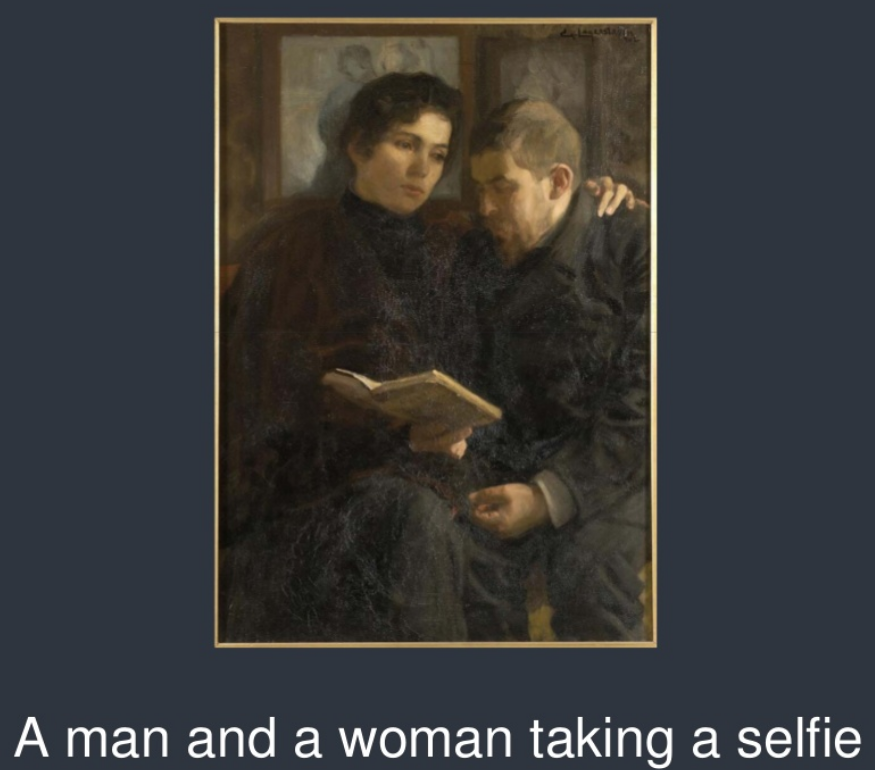
\includegraphics[width=\linewidth]{../voorstel/pictures/roddis_grappig_2}
	\end{figure}

\end{itemize}

\subsection{Computer Vision API's}
Tot slot lichten we kort CVA toe. CVA, ook wel image/visual recognition API's genoemd, zijn API's die afbeeldingen automatisch kunnen taggen (metadateren), organiseren en zoeken via machine learning. Het biedt de mogelijkheid om machine learning toe te passen zonder dat je hier zelf een expert in moet zijn. Je kan er zelf modellen mee cre\"{e}ren om de API's te trainen naar je eigen behoefte. Zo leerde Matt Fraser Google Cloud Vision verschillende spinnen te herkennen door de dienst te trainen met honderd afbeeldingen per spin~\autocite{Fraser2018}.  De bekendste diensten zijn Clarifai, IBM Visual Recognition\footnote{\url{https://www.ibm.com/watson/services/visual-recognition/}}, Microsoft Computer Vision en Google Cloud Vision.  De diensten zijn zo toegankelijk dat iedere ontwikkelaar zonder machine learning kennis modellen kan bouwen, maar dat ook, volgens TechCrunch, iedereen zonder programmeerervaring de diensten kan gebruiken om afbeeldingen te taggen en categoriseren~\autocite{Lardinois2018}. Ook uit het onderzoek van CogApp bleken de diensten eenvoudig in gebruik en precies te trainen \autocite{Hindle2017}.

%---------- Methodologie ------------------------------------------------------
\section{Methodologie}
\label{sec:methodologie}

In dit onderzoek zal bestudeerd worden of CVA helpen bij het inhoudelijk ontsluiten van erfgoedcollecties. Kunnen de ingebouwde modellen van de API's gebruikt worden, of is er nood aan (doorgedreven) training? Dit wordt onderzocht aan de hand van een prototype waarmee verschillende beelden geanalyseerd worden. Hiervoor wordt een CVA gekozen die het toelaat om eigen modellen te trainen via een webinterface, voorzien is van goede documentatie en tutorials en beschikt over API clients in een programmeertaal die gekend is door de onderzoeker (o.a. Java, Javascript, C\#). Achtereenvolgens wordt een vergelijking gemaakt tussen een set beelden die manueel beschreven werden, een set beelden die beschreven werden door de ongetrainde CVA en een set beelden die beschreven werden door een getrainde CVA.

We gebruiken hiervoor beelden van het Huis van Alijn. Het Huis van Alijn is het museum van het dagelijkse leven\footnote{\url{http///www.huisvanalijn.be}} Het museum beschikt over een grote collectie beelden die het dagelijkse leven uit de 20e eeuw documenteren. In 2011 organiseerde het museum een crowdsourcingproject waarbij foto's uit de collectie 'Anonieme snapshots' getagged konden worden om ze te beschrijven en beter toegankelijk te maken~\autocite{Wiericx2011}. Het zou interessant zijn om deze beelden te vergelijken met de resultaten van de CVA. Collectiemedewerkers van Huis van Alijn zullen mee de resultaten van de proefopstellingen analyseren en bepalen welke set van beelden voor hen over de meest bruikbare tags of metadata beschikken: de manueel beschreven beelden, de beelden getagged door de ongetrainde CVA of de beelden getagged door de getrainde CVA.
%---------- Verwachte resultaten ----------------------------------------------
\section{Verwachte resultaten}
\label{sec:verwachte_resultaten}

Van dit onderzoek worden drie resultaten verwachten.

\begin{enumerate}
\item een methodologie die door musea gebruikt kan worden om CVA in te zetten voor collectiebeschrijving. In een rapport zal beschreven worden hoe een museum CVA kan gebruiken en hoe modellen getraind kunnen worden via de webinterface en API clients. Als de CVA zo eenvoudig in gebruik zijn~\autocite{Lardinois2018}, dan zouden collectieregistratoren zelf in staat moeten zijn om de software te trainen om hen bij te staan in het ontsluiten van de collectie. Het rapport van de methodiek zal zo opgesteld worden dat de musea er zelf mee aan de slag kunnen.
\item concrete use cases die aansluiten bij de registratiepraktijk en behoeftes van een museum.
\item musea worden bewust gemaakt over het bestaan van computer vision en hoe die technologie kan bijdragen in hun werking.
\end{enumerate}

Afgaand op de resultaten uit reeds eerder gevoerd onderzoek, vermoeden we dat de CVA goed scoren op het herkennen van materiaal, het type object en de voorgestelde objecten en figuren op het object. De kwaliteit van de resultaten zal afhankelijk zijn van de specificiteit die verwacht wordt. Hoe specifieker de resultaten van de CVA moeten zijn, hoe meer de modellen getraind moeten worden.
%---------- Verwachte conclusies ----------------------------------------------
\section{Verwachte conclusies}
\label{sec:verwachte_conclusies}

CVA kan de metadata van een erfgoedobject verrijken met inhoudelijke informatie die nu niet voorkomt in de basisregistratie, zoals de sfeer en het gevoel dat op een kunstwerk weergegeven wordt en de gebruikte kleuren. Mogelijk is het zelfs in staat om bekende personen op de afbeelding te herkennen, zoals bij \textcite{Hindle2017}. Deze informatie wordt nu niet opgenomen in collectiebeheersystemen, maar is wel interessant voor onderzoekers en het publiek. We verwachten dat de meerwaarde van de CVA vooral ligt in het bijstaan van de registrator bij het inhoudelijk beschrijven. Voor collecties van het museum die momenteel niet beschreven worden door een gebrek aan personeel, tijd of budget kunnen CVA een eenvoudige manier om deze collecties toch van inhoudelijke metadata te voorzien en ze doorzoekbaar te maken.

CVA kunnen een hulp zijn bij het realiseren van een inhaalbeweging voor registratieachterstand. Er wordt verwacht dat ze de registrator kunnen ondersteunen in hun taak en informatie kunnen bezorgen die zowel voor het museum, de onderzoeker als de erfgoedge{\"i}nteresseerde interessant is. De CVA zal de registrator niet vervangen, maar kan een meerwaarde bieden aan diens werk en de registrator bijstaan bij het beschrijven van de collectie. In dit onderzoek willen we daarom aantonen wat de meerwaarde van CVA voor collectieregistratoren zijn en dat de technologie een hulpmiddel kan zijn voor collecties die niet beschreven kunnen worden.

Deze technologie zal meer en meer ingebouwd worden in DAM-systemen\footnote{Digital Asset Management Systemen, een systeem voor het opslaan, beheren en distribueren van digitale assets, zoals afbeeldingen.}. DAM-software met Computer Vision is al op de markt: Gezichtsherkenning is ingebouwd in verschillende DAM-systemen.\footnote{Zoals bij ResourceSpace: \url{https://www.resourcespace.com/knowledge-base/user/facial-recognition}}. In dit onderzoek willen we aantonen voor welke use cases deze software gebruikt kan worden in musea.

%%---------- Andere bijlagen --------------------------------------------------
% TODO: Voeg hier eventuele andere bijlagen toe
%\input{...}

%%---------- Referentielijst --------------------------------------------------

\printbibliography[heading=bibintoc]

\end{document}
